\documentclass[oneside, french, a4paper, 12pt, reqno]{book}
\usepackage[utf8]{inputenc} % Caractères spéciaux dans le code source (UTF-8)

\usepackage{tabularx}
\usepackage{tcolorbox}
\usepackage[T1]{fontenc} % Accents et caractères spéciaux
\usepackage{lmodern} % Police Latin Modern
\usepackage{xspace} % Gestion de l'espace dans les macros
\usepackage{tikz} % Package de dessin vectoriel
\usepackage{pgfplots} % Dessin de graphiques avec PGF/TikZ
  % \usepackage{cite}

% \usepackage{siunitx} % Formatage des unités et valeurs numériques
 \usepackage[arabic, main=french]{babel} % Package pour la gestion du multilinguisme (ici, français avec des caractères arabes)
\usepackage{amsmath} % Commandes et environnements mathématiques avancés
% \usepackage{amssymb} % Symboles mathématiques supplémentaires
% \usepackage{amsfonts} % Polices mathématiques supplémentaires
% \usepackage{extarrows} % Flèches mathématiques étendues
\usepackage{framed}
\usepackage[normalem]{ulem} % Soulignement et barré améliorés
\usepackage{soul} % Emphase du texte avec diverses options
\usepackage{array,ragged2e} % Gestion avancée des tableaux
\usepackage{graphicx} % Inclusion et manipulation d'images
% \usepackage{scrextend} % Options supplémentaires pour les environnements de texte
\usepackage{listings} % Environnement pour l'inclusion de code source 
\usepackage{color} % Gestion des couleurs
\usepackage[nottoc]{tocbibind} % Inclusion automatique de la table des matières dans la table des matières
\usepackage{colortbl} % Coloration des cellules de tableaux
\usepackage{subcaption} % Gestion des sous-figures et sous-tableaux
\usepackage{wrapfig} % Texte entourant les figures
\usepackage{wasysym} % Symboles additionnels
\usepackage{enumitem} % Personnalisation des listes énumérées
\usepackage{adjustbox} % Ajustement de la taille des objets
\usepackage{longtable} % Tableaux sur plusieurs pages
\usepackage{changepage} % Ajustement des marges de page localement
\usepackage{setspace} % Réglage de l'interligne
\usepackage{hhline} % Lignes horizontales améliorées dans les tableaux
\usepackage{multicol} % Texte en plusieurs colonnes
\usepackage{multirow} % Fusion de cellules dans les tableaux
\usepackage{makecell} % Personnalisation des cellules de tableau
\usepackage{tabto} % Déplacement du curseur à des positions spécifiques
\usepackage{float} % Placement précis des objets flottants
\usepackage{fancyhdr} % Personnalisation des en-têtes et pieds de page
\usepackage[toc,page]{appendix} % Gestion des annexes
 \usepackage[hidelinks]{hyperref} % Liens hypertextes
\usepackage{flowchart} % Dessin de diagrammes de flux
\usepackage[left=2.5cm,right=2.5cm,top=2.5cm,bottom=2.5cm,headheight=2.5cm]{geometry} % Mise en page des marges
\usepackage{textcomp} % Symboles de texte supplémentaires
% \usepackage{pstricks,pst-plot,pstricks-add} % Dessin avec PostScript
\usepackage{dirtytalk} % Commandes pour des guillemets améliorés
\usepackage{lipsum} % Génération de texte de remplissage (Lorem Ipsum)
%\usepackage[Glenn]{fncychap} % Personnalisation du style des chapitres
% \usepackage{tabularx}
\usepackage{array}
\usepackage{titlesec}
%\usepackage[backend=biber,style=authoryear]{biblatex} % ou un autre style
%\addbibresource{ref.bib} % <- doit être ici, dans le préambule

% hadi
% \usepackage[style=numeric,sorting=none]{biblatex}
\usepackage[style=numeric,sorting=none,backend=bibtex]{biblatex}


\addbibresource{ref.bib} % Ton fichier BibTeX

% Supprimer les dates
\AtEveryBibitem{%
  \clearfield{year}%
  \clearfield{date}%
}

% Dans le préambule
\usepackage{xcolor}
\newcommand{\HRule}{\textcolor{mycolor}{\rule{\linewidth}{0.5mm}}}


\hypersetup{pdfauthor={Nennouche}} % Nom de l'auteur

% Tikz
\usetikzlibrary{shapes.symbols,shapes.geometric,shadows,arrows.meta}
\tikzset{>={Latex[width=1.5mm,length=2mm]}}
\usetikzlibrary{calc}
% On définit quelques couleurs pour les graphiques
\definecolor{mygreen}{RGB}{28,172,0}
\definecolor{mylilas}{RGB}{170,55,241}
\definecolor{MyBlue}{HTML}{4c72b0}
\definecolor{MyGreen}{HTML}{55a868}
\definecolor{MyOrange}{HTML}{dd8452}
\definecolor{MyRed}{HTML}{c44e52}
\definecolor{mycolor}{HTML}{090482}
\definecolor{headerblue}{RGB}{200, 221, 242}
\pgfplotsset{width=10cm,compat=1.9}
\usetikzlibrary{positioning}
% On va externaliser les figures faites avec Tikz
\usepgfplotslibrary{external}
% \tikzexternalize

\TabPositions{0.49in,0.98in,1.47in,1.96in,2.45in,2.94in,3.43in,3.92in,4.41in,4.9in,5.39in,5.88in,}
\pagestyle{empty}

\urlstyle{same}

\makeatletter  % autorise l'utilisation de @
\newcommand\semiLarge{\@setfontsize\semiLarge{16}{16.5}} % Agrandir un peu plus semiLarge
\makeatother % Enlève l'utilisation de @

\renewcommand{\_}{\kern-1.5pt\textunderscore\kern-1.5pt}
\setcounter{tocdepth}{5} % Profondeur du sommaire
\setcounter{secnumdepth}{5} % Profondeur de la numérotation des sections
\setlistdepth{9} % Profondeur des listes
% On définit comment s'affichera les listes enumérées et non enumérées
\renewlist{enumerate}{enumerate}{9}
		\setlist[enumerate,1]{label=\arabic*.}
		\setlist[enumerate,2]{label=\alph*.}
\renewlist{itemize}{itemize}{9}
		\setlist[itemize,2]{label=$\circ$}
		\setlist[itemize,1]{label= -}
		\setlist[itemize,3]{label=$\ast$}
		\setlist[itemize,4]{label=$\dagger$}
		\setlist[itemize,5]{label=$\triangleright$}
		\setlist[itemize,6]{label=$\bigstar$}
		\setlist[itemize,7]{label=$\blacklozenge$}
		\setlist[itemize,8]{label=$\prime$}

\setlength{\topsep}{0pt} % Ajuste l'espacement vertical avant et après les listes
\setlength{\parskip}{9.96pt} % Ajuste l'espacement vertical entre les paragraphes
\setlength{\parindent}{0pt} % Définir l'indentation des paragraphe
%\renewcommand\bibname{Webographie} % Pour appeler les références : Bibliographie
\DefineBibliographyStrings{french}{%
  bibliography = {Webographie},
}

\renewcommand{\HRule}{\rule{\linewidth}{0.5mm}} % On définit une ligne horizontale qu'on utilisera après dans la page de garde
\renewcommand{\arraystretch}{1.3} % Ajuste l'espacement vertical des lignes dans les tableaux
% Marge et dimension du texte sur la page
\setlength{\oddsidemargin}{-1.2in}
\setlength{\topmargin}{-.2in}
\setlength{\textheight}{9.7in}
\setlength{\textwidth}{6.7in}
\geometry{hmargin=2cm,vmargin=1.5cm}
% Définir une page blanche
\newcommand\blankpage{%
    \null
    \thispagestyle{empty}%
    \addtocounter{page}{-1}%
    \newpage}
\geometry{
 a4paper,
 total={170mm,257mm},
 left=20mm,
 top=20mm,
 }
\renewcommand\headrulewidth{1pt} % Ajuste l'épaisseur de la ligne de séparation (règle) située sous l'en-tête de la page
\renewcommand{\footrulewidth}{1pt} % Ajuste l'épaisseur de la ligne de séparation (règle) située au-dessus du pied de page de la page.

\renewcommand{\sectionmark}[1]{\markboth{#1}{}}
% Pour avoir les en-tête et les pieds de pages différentes
\pagestyle{fancy}
\fancyhf{}
\rhead{\rightmark}
\lfoot{\leftmark}
\rfoot{Page \thepage}

% problème avec times pour l'afficher
\DeclareRobustCommand{\timesr}{\fontfamily{artimes}\selectfont}
\let\times\relax
\DeclareMathSymbol{\times}{\mathbin}{symbols}{"02}

% problème avec omega pour l'afficher
\DeclareRobustCommand{\omegar}{\fontfamily{aromega}\selectfont}
\let\omega\relax
\DeclareMathSymbol{\omega}{\mathord}{letters}{"21}

\titleformat{\chapter}[display]
  {\normalfont\Huge\bfseries\raggedleft}
  {Chapitre \thechapter}
  {0pt}
  {\Huge}
  
% DEBUT DU DOCUMENT
\begin{document}
    
    \topskip1pt 
    \newpage

    \rfoot{ }
        
\chapter*{Introduction générale}
\stepcounter{page}
\label{chap:intro}
\addcontentsline{toc}{chapter}{\nameref{chap:intro}}
\rhead{Introduction générale}
\setlength{\parindent}{15pt}
\rfoot{Page \thepage}
\lfoot{}
La transformation numérique des entreprises s'accompagne d'une croissance exponentielle du volume de données générées par les systèmes d'information. Dans le domaine du développement logiciel, les plateformes de suivi d'incidents telles que JIRA centralisent les signalements d'anomalies, les demandes d'amélioration et les tâches techniques. Pour les projets open source de grande envergure comme Apache Spark, qui compte près de 50 000 tickets accompagnés de millions de commentaires et d'entrées d'historique, le triage manuel de ces incidents devient difficilement soutenable.

Face à ce constat, les avancées récentes en Big Data et en intelligence artificielle offrent la possibilité de construire des plateformes capables de traiter, d'enrichir et d'analyser ces données à grande échelle, tout en produisant des prédictions exploitables.

C'est dans ce contexte que s'inscrit notre projet de fin d'études, réalisé au sein du département Data \& IA de l'agence SQLI Rabat. L'objectif est de concevoir et de mettre en œuvre une plateforme complète de triage automatique des incidents Apache Spark, reposant sur une architecture en médaillon hébergée sur Snowflake, orchestrée par dbt, et intégrant un pipeline de classification hybride combinant recherche par similarité vectorielle et arbitrage par modèle de langage via Snowflake Cortex. La plateforme produit, pour chaque ticket, une prédiction du type d'incident, une estimation de sa résolution probable et un résumé correctif exploitable par les équipes de développement.

Ce rapport documente l’ensemble du processus de développement de la solution, depuis l’analyse initiale des besoins jusqu’à sa mise en œuvre finale. Il retrace les différentes étapes qui ont jalonné ma démarche : étude du besoin, exploration de l’existant, choix des outils, conception, tests, et validation.

Il est structuré comme suit :

\begin{description}
    \item[ Chapitre 1 ] est consacré à une présentation de L’entreprise, le cadre général du stage et le parcours préparatoire réalisé en amont du projet.
    
    \item[Chapitre 2 ] présente le contexte général du projet, les objectifs visés, les spécifications fonctionnelles. Ce chapitre décrit également les outils de gestion de projet mis en place pour organiser efficacement le travail.
    
    \item[Chapitre 3 ] dresse un état de l'art des concepts et technologies liés au Big Data, en justifiant les choix technologiques retenus.
    
    \item[Chapitre 4 ] est dédié à la conception de la solution, incluant l’architecture technique, les choix de modélisation, et les flux de traitement.
    
    \item[Chapitre 5 ] décrit la réalisation et la mise en œuvre, en présentant l'implémentation détaillée et les résultats obtenus.
\end{description}

        \chapter{Cadre général du stage et parcours préparatoire}
    
\rhead{Cadre général du stage et parcours préparatoire}
\lfoot{\leftmark}

\section{Introduction}
Ce chapitre présente le cadre général du stage de fin d'études. Nous commençons par une présentation de l'organisme d'accueil, le groupe SQLI, avant de détailler le parcours d'intégration et les activités préliminaires réalisées en amont du projet.

%--------------------------SQLI------------------------------
\section{Présentation de l'organisme d'accueil}
\subsection{Groupe SQLI}
Fondé en 1990, SQLI est un groupe européen de services digitaux spécialisé dans la conception d’expériences digitales innovantes. Il accompagne de grandes marques internationales dans leur transformation numérique, en les aidant à créer de la valeur à travers le digital.

Le groupe SQLI compte près de 3 400 collaborateurs répartis dans plusieurs pays, notamment en France (Paris, Lyon, Toulouse, Bordeaux, Rouen, Nantes, Lille), en Suisse(Lausanne, Genève), au Luxembourg, en Belgique (Bruxelles), aux Pays-Bas, au Maroc(Rabat, Casablanca, Oujda), ainsi qu’en Espagne (Barcelone) et à Dubaï.

Le groupe accorde une importance particulière aux méthodologies agiles, et conduit la majorité de ses projets selon le cadre SCRUM. Cette organisation agile contribue à sa performance, avec un chiffre d’affaires ayant atteint 251,2 millions d’euros en 2023, en constante progression depuis plusieurs années. \cite{logo:sqli1}

SQLI compte plus de 2000 clients, grands comptes et PME, issus de divers secteurs d’activité, tels que :
\begin{itemize}
    \item Les services
    \item Les banques et assurances
    \item Les administrations et services publics
    \item La distribution
    \item L’immobilier
    \item Les transports
    \item Les télécommunications
\end{itemize}

La figure 1.1 présente la répartition de SQLI dans le monde.

\begin{figure}[H]
    \centering
    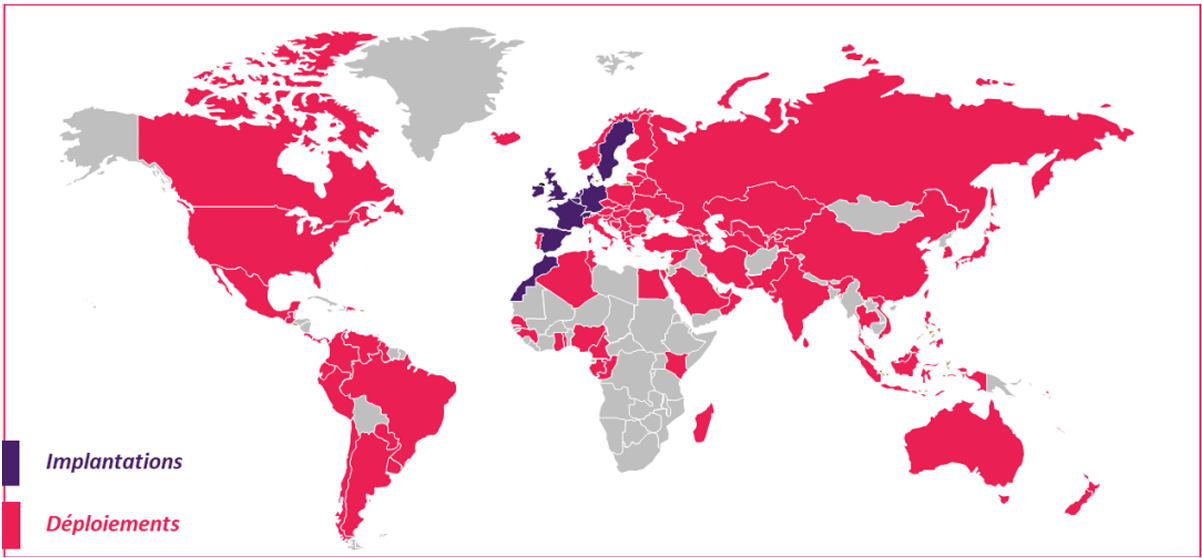
\includegraphics[width=1\textwidth]{images/sqlirepartition.png}
    \caption{Présence de SQLI dans le monde}
\end{figure}

\subsection{Fondamentaux SQLI}
L'agence SQLI Rabat dispose d'un département Data \& IA, qui regroupe des expertises en data engineering, data science et en analyse avancée des données pour répondre aux besoins métiers. L'agence mobilise une grande diversité de technologies pour accompagner ses clients, tout en partageant les mêmes fondamentaux organisationnels et humains que l'ensemble du groupe SQLI.

SQLI place au cœur de sa culture d'entreprise des valeurs fortes telles que le respect, l'esprit d'équipe, l'authenticité, l'engagement et le goût du challenge. Les collaborateurs sont encouragés à innover, à proposer des idées et à s'impliquer activement dans les projets.

Trois axes majeurs structurent la démarche du groupe :
\begin{itemize}
    \item L’excellence opérationnelle, appuyée par la méthodologie CMMI, avec une certification de niveau 3 obtenue dès 2006.
    \item La relation client, fondée sur l’écoute et la compréhension des enjeux métiers, à travers le programme qualité interne Business CMM.
    \item L’innovation, portée par le laboratoire interne 6mmx, qui conçoit des solutions performantes et génératrices de valeur, déployées à l’échelle du groupe.
\end{itemize}

\subsection{Organigramme de Sqli}
Lasociété SQLI dispose d’un organigramme illustrant sa structure globale et l’organisation de ses différents services.

Autrefois indépendants, les centres de Rabat et Oujda ont récemment été fusionnés dans le cadre d’une nouvelle réorganisation interne, donnant naissance à une entité unique : ISC Maroc (Industrialized Services Center).

Cette restructuration vise à renforcer la synergie entre les équipes et à offrir une vision plus cohérente et centralisée de l’organisation.

La figure \ref{fig:organi} présente l’organigramme adopté par SQLI
\begin{figure}[H]
    \centering
    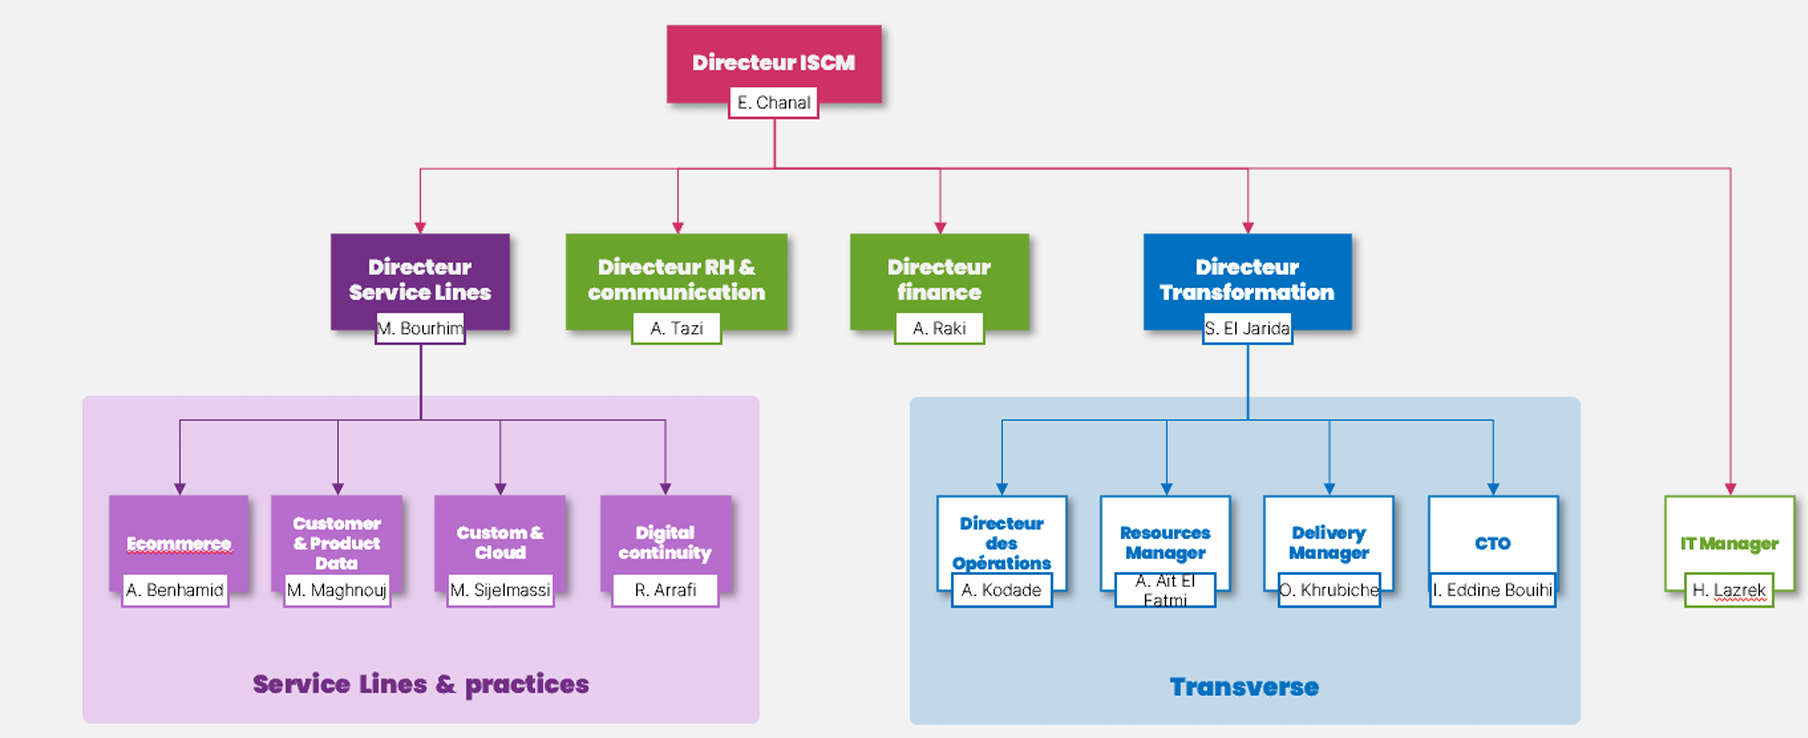
\includegraphics[width=1\textwidth]{images/organigramme.png}
    \caption{Organigramme de SQLI}
    \label{fig:organi}
\end{figure}

\subsection{Mission et domaines d’expertise}
SQLI a pour mission de créer des expériences digitales à forte valeur ajoutée pour les grandes marques, en les accompagnant dans leur transformation numérique. Le groupe se distingue par son approche centrée sur l’innovation et l’expérience utilisateur, en proposant des solutions adaptées aux besoins spécifiques de chaque client.

SQLI intervient dans plusieurs domaines clés :
\begin{itemize}
    \item \textbf{E-commerceetExpériences Digitales: } Création de plateformes e-commerce, sites web interactifs, et applications mobiles. 
    \item \textbf{Data et Intelligence Artificielle: } Exploitation des données pour améliorer la performance des entreprises grâce à l’analyse de données, l’automatisation, et le machine learning.
    \item \textbf{Stratégie Digitale: }  Conseil et accompagnement dans la définition et la mise en œuvre de stratégies digitales pour améliorer la compétitivité.
    \item \textbf{Transformation Digitale: }  Intégration de nouvelles technologies et optimisation des processus pour une meilleure efficacité opérationnelle.
\end{itemize}

\subsection{Partenaires de SQLI}
SQLI s’appuie sur un réseau de partenaires technologiques stratégiques afin d’enrichir son offre de services et de garantir à ses clients des solutions performantes, innovantes et adaptées aux standards du marché.
La figure \ref{fig:part} représente les logos de quelques
partenaires technologiques de SQLI. \cite{logo:sqli2}
\begin{figure}[H]
    \centering
    
\includegraphics[width=1\textwidth]{images/partenaires.png}
    \caption{Logos des principaux partenaires de SQLI}
    \label{fig:part}
\end{figure}
%------------------------------Activités--------------------------
\section{Intégration et activités préliminaires}
Chaque année, SQLI organise le concours national e-Challenge, un événement destiné à renforcer les liens entre l’entreprise et les établissements d’enseignement supérieur. Cette initiative a pour but d’offrir aux futurs lauréats une immersion concrète dans le monde
professionnel, à travers la réalisation de projets de fin d’études (PFE) avec une réelle perspective d’embauche.

Dans ce cadre, le processus de sélection débute par un concours technique sur la plateforme HackerRank, consistant en une épreuve de 3 heures axée sur des problématiques
d’algorithmique, de développement et de logique. Les candidats retenus passent ensuite un entretien technique et RH, d’une durée d’environ une heure, afin d’évaluer à la
fois leurs compétences techniques et leur adéquation avec les valeurs de l’entreprise.
\subsection{Formation sur les technologies Big Data et Cloud }
À l'issue du processus de sélection, les candidats admis bénéficient d'un programme de formation intensif d'une durée de quatre semaines, dispensé via la plateforme Udemy. Cette formation vise à consolider les compétences techniques nécessaires au bon déroulement du stage, en couvrant les technologies clés de l'écosystème Data \& IA de l'entreprise.

Le programme s'articule autour de quatre modules complémentaires. 
\begin{itemize}
    \item Le premier module consiste en un bootcamp complet en SQL et Snowflake, axé sur les fondamentaux de l'analyse de données, notamment la manipulation de requêtes complexes et l'exploitation des fonctionnalités avancées de Snowflake.
    \item Le deuxième module est consacré à l'analyse de données avec Pandas et Python, permettant de maîtriser le traitement, le nettoyage et la transformation de jeux de données volumineux.
    \item Le troisième module porte sur Azure Databricks et Spark SQL avec Python, offrant une introduction à l'environnement cloud Azure ainsi qu'au traitement distribué des données à grande échelle.
    \item Le quatrième module constitue une formation avancée sur Snowflake, couvrant l'ensemble de ses fonctionnalités, de l'architecture interne à l'optimisation des performances.
\end{itemize}
Ce parcours de formation a permis d'acquérir une maîtrise solide des outils et technologies mobilisés tout au long du projet de fin d'études, tout en facilitant l'intégration au sein de l'équipe Data \& IA de l'agence.

\subsection{Préparation à la certification Snowflake}
En parallèle du programme de formation, une phase de préparation à la certification SnowPro Core (C03) a été engagée. Cette certification, délivrée officiellement par Snowflake, atteste d'un niveau de compétence solide sur les concepts fondamentaux de la plateforme, couvrant notamment l'architecture, le chargement et la transformation des données, la gestion des entrepôts virtuels, la sécurité ainsi que l'optimisation des performances.

La préparation s'est appuyée sur plusieurs ressources complémentaires. Les connaissances acquises lors des modules de formation Udemy, en particulier les deux modules dédiés à Snowflake, ont constitué une base essentielle. Cette base a été renforcée par l'étude approfondie de la documentation officielle de Snowflake, ainsi que par la réalisation de nombreux examens blancs permettant de se familiariser avec le format des questions et d'identifier les axes d'amélioration.

Cette démarche a abouti à l'obtention de la certification SnowPro Core (C03), validant ainsi une maîtrise des fonctionnalités clés de la plateforme Snowflake. Cette certification représente un atout significatif dans le cadre du projet de fin d'études, dans la mesure où Snowflake constitue l'un des piliers technologiques de la solution mise en œuvre.

La figure \ref{fig:certisnow} présente une copie du certificat obtenu.
\begin{figure}[H]
    \centering
    
\includegraphics[width=1\textwidth]{images/certifsnow.png}
    \caption{Certificat SnowPro Core (C03)}
    \label{fig:certisnow}
\end{figure}

\subsection{Participation au Hackathon}
Dans le cadre des activités préliminaires au stage, une participation à un hackathon interne organisé par SQLI a été réalisée. Cet événement portait sur l'utilisation de Snowflake Cortex et s'inscrivait dans le contexte d'un cas d'usage réel pour un client majeur de l'entreprise.

Le hackathon était structuré en deux volets complémentaires. Le premier volet, orienté Data Engineering, consistait à mettre en place les pipelines de préparation et de transformation des données nécessaires à l'alimentation de la solution. Le second volet, dédié à l'intelligence artificielle, portait sur l'exploitation des modèles de langage avancés (LLM) intégrés à Snowflake Cortex afin d'automatiser des tâches complexes, notamment l'analyse et la prédiction.

L'objectif était de concevoir une solution complète de traitement et d'analyse intelligente des incidents, en s'appuyant sur une approche de Root Cause Analysis (RCA) appliquée aux tickets JIRA. Cette solution visait à identifier automatiquement les causes profondes des incidents récurrents, réduisant ainsi le temps de diagnostic et améliorant la prise de décision.

Cette expérience a constitué une mise en pratique concrète des compétences acquises lors de la formation, tout en offrant une première confrontation avec les exigences d'un projet réel en environnement professionnel.

La figure \ref{fig:certihackath} présente une copie du certificat de participation à ce hackathon.
\begin{figure}[H]
    \centering
    
\includegraphics[width=1\textwidth]{images/hackathon.jpeg}
    \caption{Certificat de participation au hackathon}
    \label{fig:certihackath}
\end{figure}

\subsection{Compétences acquises}
L'ensemble des activités préliminaires menées au cours de cette phase d'intégration a permis de développer un socle de compétences à la fois techniques et transversales, directement mobilisables dans le cadre du projet de fin d'études.

Sur le plan technique, les compétences acquises couvrent plusieurs domaines clés. La maîtrise de la plateforme Snowflake, validée par l'obtention de la certification SnowPro Core (C03), constitue un acquis majeur, englobant l'architecture cloud, la gestion des entrepôts virtuels, le chargement et la transformation des données ainsi que l'optimisation des performances. La formation a également permis de consolider les compétences en SQL avancé pour l'interrogation et l'analyse de données complexes, en Python appliqué à la manipulation de données à travers la bibliothèque Pandas, ainsi qu'en traitement distribué via Apache Spark SQL sur l'environnement Azure Databricks. Par ailleurs, la participation au hackathon a offert une première expérience pratique avec les modèles de langage intégrés à Snowflake Cortex.

Sur le plan transversal, cette phase a favorisé le développement de compétences en travail collaboratif et en gestion du temps, notamment lors du hackathon où la coordination au sein de l'équipe et le respect des délais étaient essentiels. La capacité à appréhender rapidement de nouvelles technologies et à les appliquer dans un contexte concret a également été renforcée, de même que l'aptitude à analyser une problématique métier et à proposer une solution adaptée.

Ces compétences constituent un socle solide pour aborder le projet de fin d'études dans les meilleures conditions.

\section{Conclusion}
Ce chapitre a permis de présenter l'organisme d'accueil ainsi que le parcours préparatoire au stage, incluant la formation, la certification SnowPro Core (C03) et la participation au hackathon. Ces étapes ont constitué une base solide pour aborder le projet de fin d'études, dont le contexte général sera détaillé dans le chapitre suivant.
        \chapter{Contexte général du projet}
    
\rhead{Contexte général du projet}
\lfoot{\leftmark}

\section{Introduction}
Ce chapitre a pour objectif de définir le cadre dans lequel s'inscrit le projet de fin d'études. Nous commençons par présenter le contexte général et la problématique à laquelle répond le projet, avant de détailler la solution proposée, les objectifs visés, les livrables attendus ainsi que les spécifications des besoins. Enfin, nous abordons la méthodologie adoptée et la planification du projet.

%--------------------------1-----------------------------
\section{Contexte du projet}
Le projet Apache Spark \cite{logo:apache_spark}, géré via la plateforme JIRA \cite{logo:jira_apache} de la fondation Apache, figure parmi les initiatives open source les plus dynamiques dans l'écosystème du traitement distribué. Au fil des années, ce projet a généré un volume considérable de tickets, avoisinant les 50 000 entrées, de natures très diverses : signalements d'anomalies, demandes d'amélioration, ajouts de fonctionnalités, tâches techniques, sous-tâches, interrogations ou encore éléments de documentation. Chacun de ces tickets s'accompagne d'un ensemble dense de métadonnées : un intitulé synthétique, un descriptif parfois très long, des fils de commentaires, un journal de modifications traçant chaque changement de champ, des liaisons vers d'autres tickets, sans oublier les informations relatives à la priorité, au statut courant, à la personne ayant signalé le problème et à celle chargée de le traiter.

Dans un tel environnement, l'activité de triage, c'est-à-dire la catégorisation et l'orientation de chaque nouveau ticket, représente un enjeu opérationnel majeur. Il s'agit concrètement de déterminer la nature exacte du ticket, d'estimer comment il sera vraisemblablement résolu et de formuler une piste d'action pour les développeurs. Aujourd'hui, cette tâche incombe principalement à des contributeurs expérimentés qui l'effectuent manuellement, ce qui consomme un temps non négligeable et reste exposé aux aléas de l'interprétation humaine, surtout lorsque le flux de tickets s'intensifie.

% Notre travail prolonge l'expérience acquise lors du hackathon Data \& IA organisé par SQLI, au cours duquel une première approche de triage hybride a été explorée à l'aide de Snowflake Cortex. L'ambition est ici de passer d'un prototype à une plateforme industrialisée et enrichie. Les données exploitées proviennent d'un export public du JIRA Apache Spark, mis à disposition sur Kaggle en mars 2025. Cet export totalise environ 49 832 tickets pour le projet SPARK, auxquels sont associés plus de cinq millions de commentaires, 9,6 millions d'entrées dans le journal de modifications et 390 000 relations entre tickets.

%------------------------2--------------------------
\section{Étude de l’existant}
Plusieurs stratégies ont été documentées dans la littérature et dans la pratique pour aborder la question du triage automatique des incidents logiciels. Nous en distinguons quatre grandes familles.
\begin{itemize}
    \item La première, et la plus couramment observée dans les projets open source de grande envergure, est le triage entièrement manuel. Des contributeurs chevronnés parcourent les tickets un par un, les catégorisent selon leur expérience et les affectent aux personnes compétentes. Si cette méthode bénéficie d'une connaissance fine du contexte technique, elle présente des faiblesses structurelles : le temps consacré à chaque ticket est élevé, la disponibilité des experts conditionne le rythme de traitement, les critères de classification varient d'un triageur à l'autre, et les épisodes de forte affluence engendrent des retards cumulatifs.
    \item La deuxième famille regroupe les techniques d'apprentissage automatique supervisé dites classiques. Des algorithmes tels que les séparateurs à vaste marge, les ensembles d'arbres de décision ou les classifieurs probabilistes sont alimentés par des vecteurs de caractéristiques construits manuellement à partir du texte des tickets, par exemple via des représentations en sacs de mots ou en pondérations TF-IDF \cite{logo:tfidf}. Ces méthodes ont produit des résultats intéressants sur des corpus de taille modeste, mais elles peinent à saisir les nuances sémantiques des descriptions techniques et exigent un investissement conséquent dans la phase de construction des caractéristiques.
    \item La troisième famille s'appuie sur les grands modèles de langage. Grâce à leur capacité à appréhender le sens contextuel de textes spécialisés, ces modèles offrent des performances de classification et de génération nettement supérieures. Toutefois, leur mise en œuvre directe pour le triage soulève des questions de coût computationnel, de temps de réponse et de contrôle de la qualité des sorties, notamment lorsqu'il faut garantir des prédictions cohérentes sur des milliers de tickets.
    \item La quatrième famille, qualifiée d'hybride, associe une recherche par similarité vectorielle à un arbitrage par modèle de langage, selon le principe du Retrieval-Augmented Generation (RAG) \cite{logo:rag}. Son intérêt réside dans la complémentarité entre la rapidité de la recherche par plus proches voisins et la finesse de raisonnement du modèle de langage, le tout encadré par un mécanisme de seuil de confiance qui réserve les appels coûteux au LLM aux seules situations véritablement ambiguës.
\end{itemize}

Au terme de cette analyse, il ressort qu'aucune solution opérationnelle ne fédère dans une même architecture l'ensemble de la chaîne nécessaire : ingestion, transformation, enrichissement par des indicateurs issus de l'historique de modifications et des relations inter-tickets, classification hybride et production d'analyses correctives, le tout hébergé sur une plateforme cloud unifiée.

%------------------------3-------------------------
\section{Problématique}
Le processus de triage des incidents du projet Apache Spark repose, dans sa forme actuelle, sur une intervention humaine systématique. Les responsables qualité doivent lire chaque ticket dans son intégralité, en identifier la nature, projeter son issue probable et orienter les équipes de développement. Avec un historique de près de 50 000 tickets et un flux continu de nouvelles entrées, cette organisation atteint ses limites. Nous identifions trois difficultés majeures.

\begin{itemize}
    \item La première touche au coût temporel du diagnostic. L'examen approfondi d'un ticket complexe, englobant sa description, ses commentaires et l'intégralité de son journal de modifications, peut s'avérer particulièrement chronophage, a fortiori lorsque le ticket a fait l'objet de multiples réassignations ou d'escalades de priorité.
    \item La deuxième difficulté concerne l'hétérogénéité des classifications. Sans règles formalisées ni assistance automatisée, deux triageurs confrontés au même ticket peuvent aboutir à des catégorisations divergentes, ce qui nuit à la cohérence du suivi et fausse l'analyse des tendances sur le long terme.
    \item La troisième difficulté porte sur la sous-exploitation des métadonnées disponibles. Le journal de modifications recèle des informations précieuses, telles que la fréquence des transitions de statut, les hausses de priorité ou la diversité des intervenants, qui constituent autant d'indices sur la complexité et la criticité d'un ticket. Or, ces signaux ne sont aujourd'hui intégrés dans aucune démarche de triage existante.
\end{itemize}

La question centrale à laquelle ce projet entend répondre est la suivante : comment élaborer et déployer une plateforme intégrée permettant d'automatiser le triage des incidents Apache Spark, en valorisant la totalité des données JIRA disponibles, dans le but de prédire la catégorie de l'incident et son issue probable, tout en proposant une analyse corrective directement exploitable par les équipes ?

%------------------------4-------------------------
\section{Solution proposée}
Pour répondre à cette problématique, nous proposons la conception et le déploiement d'une plateforme de triage automatique reposant sur une architecture en médaillon à trois niveaux (Bronze, Argent, Or) \cite{logo:medallion}, hébergée intégralement sur Snowflake \cite{logo:snowflake} et orchestrée par dbt \cite{logo:dbt}.

La couche Bronze prend en charge l'ingestion fidèle des données brutes issues des fichiers CSV sources, sans aucune transformation métier, afin de préserver l'intégralité de l'information d'origine.

La couche Argent porte l'essentiel de la logique de transformation. Elle assure le filtrage, le nettoyage textuel, la consolidation des étiquettes en catégories exploitables, le partitionnement temporel des données, ainsi que l'extraction de caractéristiques originales à partir du journal de modifications et des relations entre tickets. Ces caractéristiques constituent l'apport technique distinctif de ce projet.

La couche Or produit les tables de consommation finales, alimentant d'une part le pipeline de classification et d'autre part le tableau de bord analytique.

Le moteur de classification s'appuie sur une approche hybride combinant une recherche par similarité vectorielle avec un arbitrage par modèle de langage lorsque le niveau de confiance est insuffisant. Ce pipeline produit, pour chaque ticket, une prédiction du type d'incident, une prédiction de la résolution probable et un résumé correctif court.

La plateforme expose deux canaux de restitution : une application de triage en temps réel développée avec Streamlit \cite{logo:streamlit}, et un tableau de bord analytique multi-pages permettant l'exploration des données opérationnelles. Les détails de conception et d'implémentation de chacune de ces couches seront approfondis dans les chapitres suivants.

%------------------------5-------------------------
\section{Objectifs du projet}
Ce projet poursuit un objectif principal et plusieurs objectifs spécifiques.

L'objectif principal est de concevoir et de mettre en service une plateforme de bout en bout automatisant le triage des incidents Apache Spark, couvrant l'intégralité de la chaîne, depuis l'ingestion des données brutes jusqu'à la restitution des prédictions et des analyses.
Pour les objectifs spécifiques
\begin{itemize}
    \item Le premier consiste à bâtir une architecture en médaillon fiable sur Snowflake, pilotée par dbt, dans laquelle chaque transformation est tracée et validée par des tests automatisés.
    \item Le deuxième vise à extraire et intégrer des caractéristiques inédites issues du journal de modifications et des liaisons entre tickets. 
    \item Le troisième objectif porte sur le calibrage du pipeline de classification hybride pour dépasser un taux de classification correcte de 70 \% sur le type d'incident et de 75 \% sur la résolution. 
    \item Le quatrième objectif consiste à développer une interface de triage en temps réel et un tableau de bord d'analyse accessibles aux responsables qualité.
    \item Le cinquième objectif est d'assurer la reproductibilité intégrale de la solution au moyen d'une documentation exhaustive et d'un déploiement par conteneurs.
\end{itemize}
%------------------------6-------------------------
\section{Livrables attendus}
Le projet doit aboutir à la production de sept livrables distincts.
\begin{itemize}
    \item Le premier est la base de données Snowflake organisée selon l'architecture en médaillon, comprenant six schémas dédiés aux différentes couches de transformation et de consommation.
    \item Le deuxième est le projet dbt dans son intégralité, englobant les modèles de transformation pour chaque couche, les tables de correspondance pour le regroupement des étiquettes, les macros de nettoyage textuel et la batterie de tests automatisés.
    \item Le troisième est le pipeline V6 Hybrid RCA, matérialisé par quatre scripts SQL séquentiels couvrant l'enrichissement, le calcul des représentations vectorielles, la prédiction et l'évaluation.
    \item Le quatrième est l'application de triage en temps réel, développée avec Streamlit, offrant pour chaque ticket soumis une prédiction du type, de la résolution et un résumé correctif.
    \item Le cinquième est le tableau de bord analytique multi-pages, permettant l'exploration des données opérationnelles et des relations entre tickets.
    \item Le sixième est la documentation technique, comprenant le dictionnaire des données, le journal des décisions architecturales et le schéma global de la plateforme.
    \item Le septième est l'environnement de déploiement conteneurisé, permettant le lancement de l'ensemble des applications par une commande unique.
\end{itemize}

%------------------------7-------------------------
\section{Spécification des besoins}
\subsection{Besoins fonctionnels}
 la plateforme doit être capable d'ingérer les données JIRA Apache Spark depuis des fichiers CSV et de les charger dans Snowflake en préservant l'intégralité de l'information. Elle doit appliquer aux données brutes un traitement comprenant un nettoyage textuel, une consolidation des étiquettes et un partitionnement temporel. Elle doit calculer des indicateurs à partir du journal de modifications, notamment le nombre de transitions de statut, les variations de priorité, les changements d'assignataire, la détection des escalades et le dénombrement des intervenants uniques. Elle doit également dériver des indicateurs à partir des relations entre tickets, incluant les doublons, les blocages et les liens de type informationnel. La plateforme doit attribuer à chaque ticket une catégorie parmi neuf classes de type et une parmi sept classes de résolution. Elle doit produire un résumé correctif concis pour chaque prédiction. Elle doit mettre à disposition une interface de triage en temps réel pour un ticket individuel, ainsi qu'un tableau de bord interactif couvrant les dimensions opérationnelles et relationnelles des tickets.

\subsection{Besoins non fonctionnels}
la plateforme doit garantir un taux de classification correcte dépassant 70 \% pour le type d'incident et 75 \% pour la résolution. La fiabilité des transformations doit être assurée par des tests dbt automatisés portant sur l'unicité des clés, l'absence de valeurs manquantes sur les champs critiques, le respect des valeurs autorisées et la cohérence des relations entre tables. La confidentialité doit être respectée en maintenant une version locale de développement séparée de l'environnement de production de l'entreprise. L'ensemble de la solution doit pouvoir être reproduit et déployé via un système de conteneurisation. Le pipeline principal de classification doit s'appuyer exclusivement sur les modèles accessibles via Snowflake Cortex, sans recourir à des services tiers. Enfin, le code source et la documentation doivent faire l'objet d'un suivi de versions sur un dépôt distant.

%------------------------8-------------------------
\section{Méthodologie et gestion du projet}
\subsection{Choix de la méthode de gestion du projet}

La conduite du projet s'appuie sur une démarche itérative et incrémentale, inspirée du cadre Scrum tel que pratiqué au sein de SQLI. Ce choix permet de livrer progressivement les différentes briques de la plateforme, en ménageant à chaque itération des moments de revue et d'ajustement avec l'encadrant en entreprise.

Le processus Scrum\cite{logo:SCRUM}, représenté à la Figure~\ref{fig:scrum}, suit les étapes suivantes :

\begin{description}
    \item[Identification des fonctionnalités] à développer pour construire le backlog produit (ingestion des fichiers CSV dans Snowflake, nettoyage et transformation des données via dbt, extraction des features du changelog et des liens entre tickets, mise en place du pipeline de classification hybride, développement de l'application d'inférence Streamlit, création du tableau de bord analytique, conteneurisation via Docker).
    \item[Priorisation des tâches] à travers des sprints successifs, en tenant compte de la complexité technique et des dépendances entre composants.
    \item[Développement itératif] où chaque sprint aboutit à un incrément fonctionnel du produit, tel qu'une couche Bronze opérationnelle avec tests de validation, un pipeline dbt complet produisant la table mart_ml, un premier prototype du pipeline de classification ou encore un tableau de bord avec les premières visualisations.
\end{description}

Cette approche m'a permis de progresser de façon organisée et adaptable, en passant par des étapes bien définies telles que la planification des tâches, le développement itératif et les tests, ainsi que l'intégration continue des composants. 

\begin{figure}[H]
    \centering
    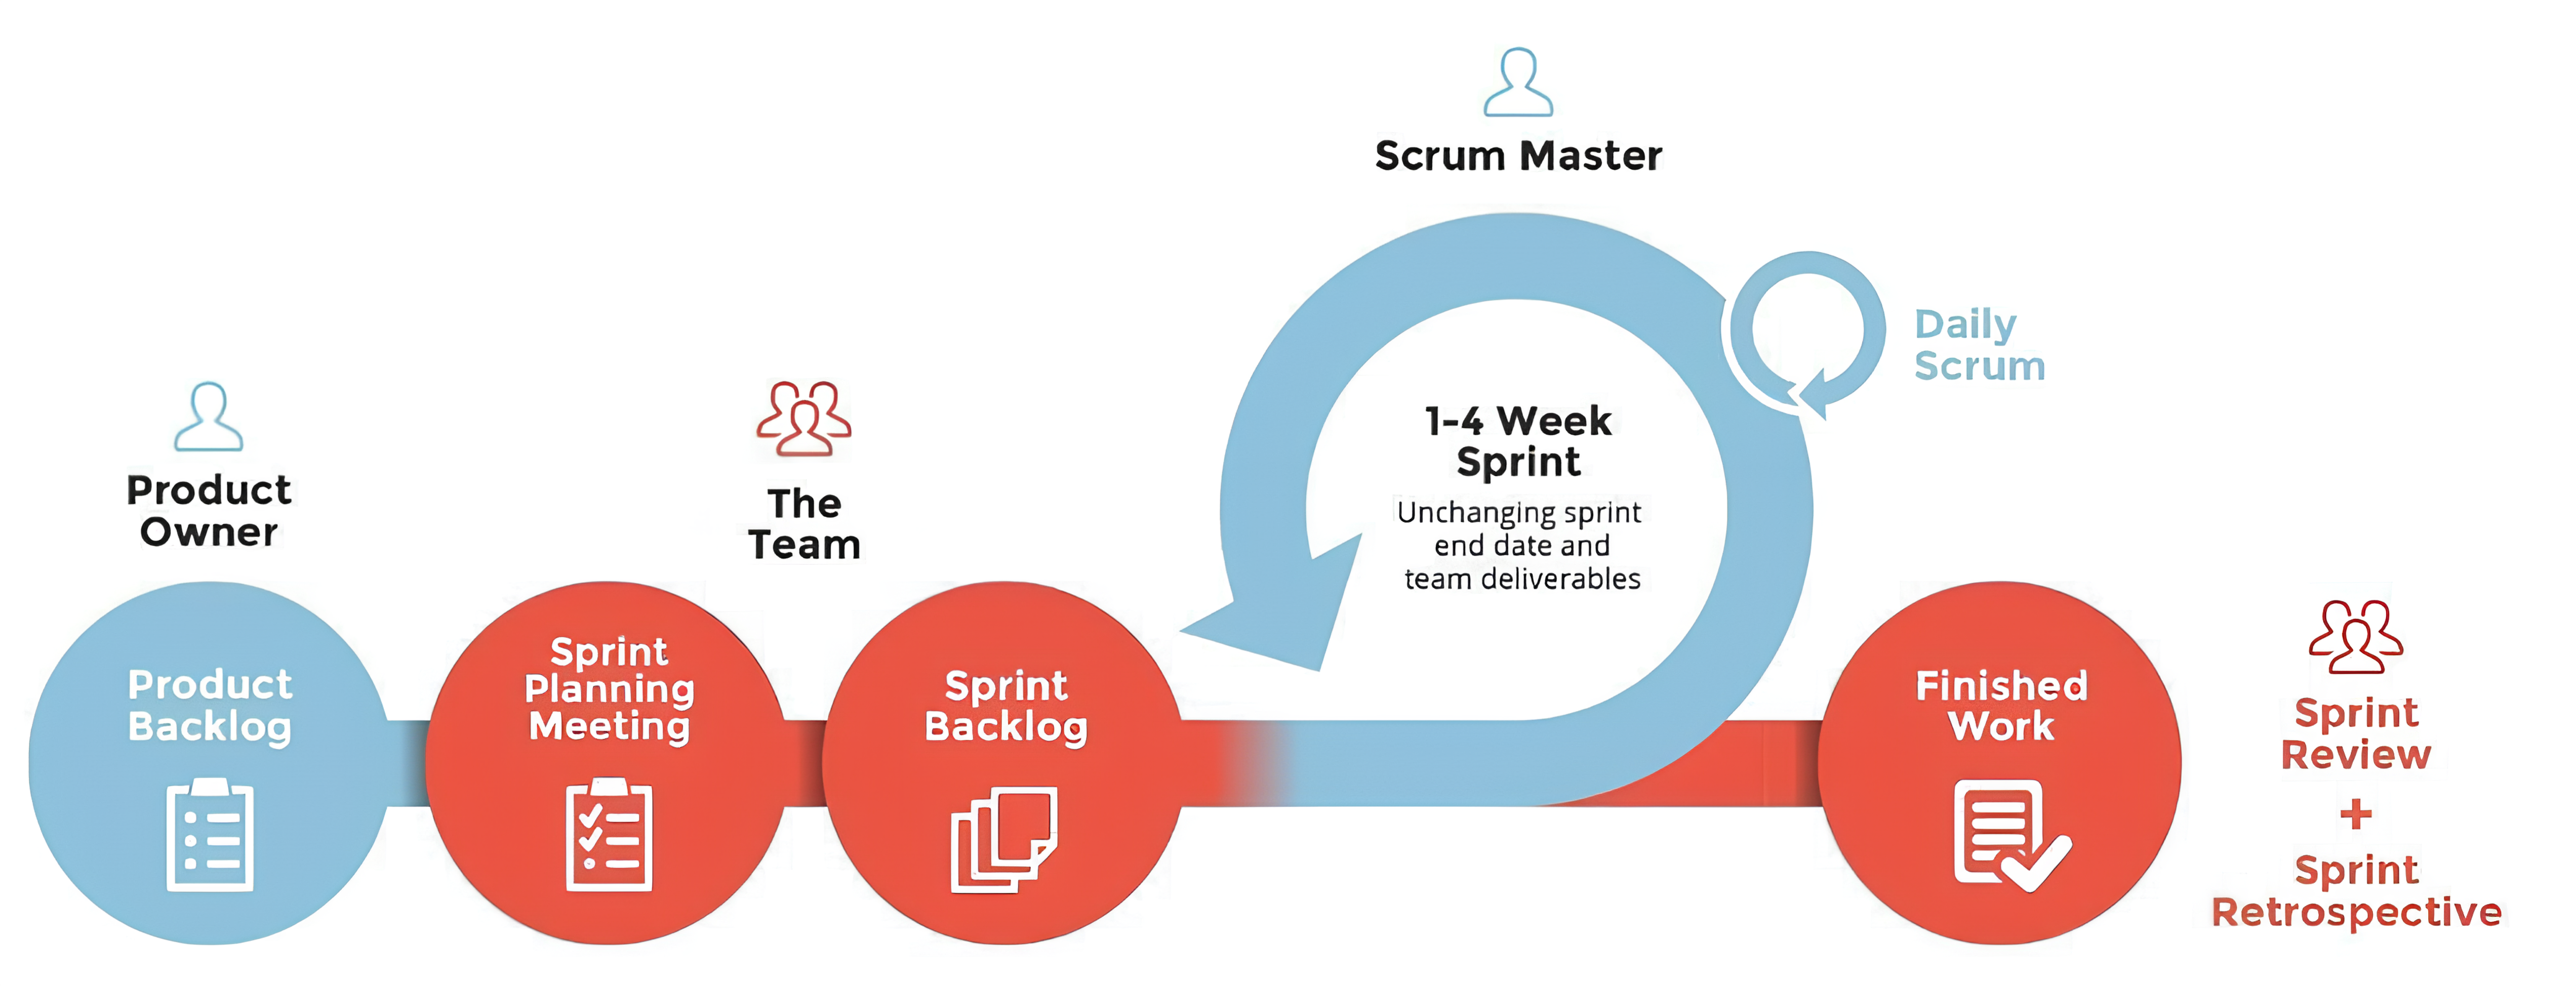
\includegraphics[width=1\textwidth]{images/scrum.png}
    \caption{Processus de SCRUM}
    \label{fig:scrum}
\end{figure}

% \subsection{Equipes et rôles}

% La répartition des rôles au sein de l’équipe projet, selon l’approche Scrum, est présentée dans le tableau \ref{tab:equipe_roles}.\\

% \begin{minipage}{1\textwidth}
%     \centering
% \begin{tabular}{|c|>{\raggedright\arraybackslash}p{10cm}|}
%   \hline
%   Product Owner &  \\
%   \hline
%   Scrum Master &  \\
%   \hline
%   L'équipe de développement & 
%    \\
%   \hline
% \end{tabular}
% \captionof{table}{Équipes et rôles}
% \label{tab:equipe_roles}
% \end{minipage}

\subsection{Planification du projet}
La phase de planification revêt une importance capitale dans la préparation d’un projet. Elle implique l’identification et la planification des différentes tâches du projet, ainsi que l’estimation de leur charge de travail respective. 

Le découpage temporel du projet en sprints, ainsi que les activités principales associées à chaque phase, sont présentés dans le tableau \ref{tab:planification}.

\begin{table}[h!]
\centering
\begin{tabularx}{\textwidth}{|c|X|}
  \hline
  \textbf{Période} & \textbf{Sprint / Activités} \\
  \hline
  2 semaines & Sprint 1 : Prise en main du sujet et compréhension du besoin  \\
  \hline
  1 semaine & Sprint 2 : Ingestion et couche Bronze \\
  \hline
  1 semaine & Sprint 3 : Transformation et couches Argent/Or  \\
  \hline
  2 semaines & Sprint 4 : Pipeline de classification et inférence  \\
  \hline
  1 semaines & Sprint 5 : Visualisation des données  \\
  \hline
  1 semaines & Sprint 6 : Phase de test et validation des résultats \\
  \hline
\end{tabularx}
\caption{Planification du projet}
\label{tab:planification}
\end{table}

\subsection{Synthèse visuelle}
\subsubsection{Diagramme de GANTT}
La planification globale du projet, incluant la répartition des tâches dans le temps, est visualisée à travers le diagramme de Gantt présenté à la figure \ref{fig:gantt}. Ce dernier constitue l’un des outils les plus efficaces pour représenter l’état d’avancement des différentes tâches qui composent un projet. Les unités de temps (jours, semaines, mois) sont indiquées en haut du diagramme, tandis que toutes les tâches à accomplir apparaissent dans la colonne de gauche. Chaque tâche est représentée par une barre horizontale dont la position et la longueur indiquent respectivement la date de début, la durée et la date de fin. Ce diagramme permet ainsi de visualiser clairement l’enchaînement des activités, leur durée, ainsi que les dates clés du projet.

\begin{figure}[H]
    \centering
    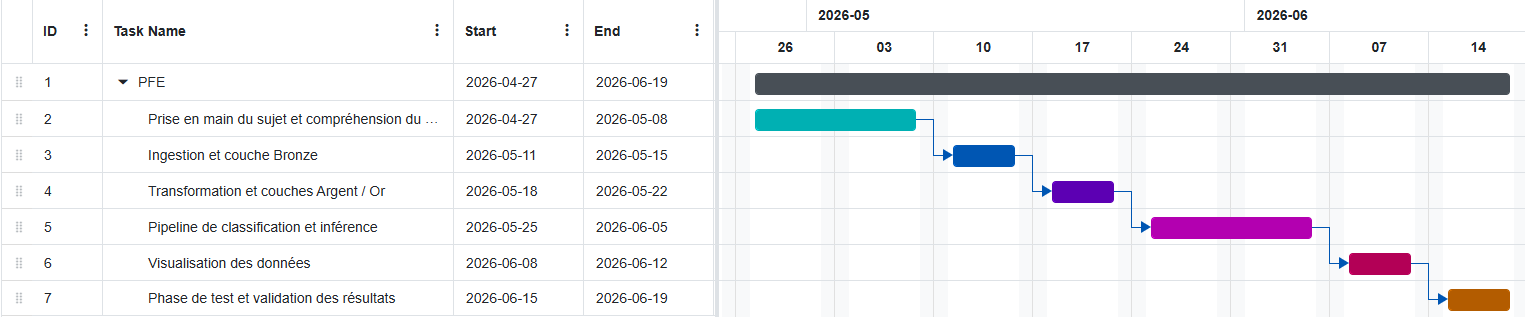
\includegraphics[width=1\textwidth]{images/gantt.png}
    \caption{Diagrmme de Gantt}
    \label{fig:gantt}
\end{figure}

%------------------------9-------------------------

\section{Conclusion}
Ce chapitre a permis de délimiter le périmètre du projet en posant le contexte métier, en analysant les approches existantes et en formulant la problématique à laquelle nous répondons. La solution retenue, ses objectifs, ses livrables et ses exigences ont été exposés de manière détaillée, et la démarche de conduite du projet a été établie. Dans le chapitre suivant, nous dresserons un état de l'art des concepts et technologies liés au Big Data, en justifiant les choix techniques retenus pour la réalisation de la plateforme

        \chapter{État de l'art}

\rhead{État de l'art}
\lfoot{\leftmark}

\section{Introduction}
Ce chapitre dresse un panorama critique des technologies, des paradigmes et des travaux de recherche qui constituent le fondement théorique et pratique de notre projet. L'automatisation du triage de tickets logiciels est un problème à l'intersection de plusieurs domaines : l'ingénierie des données à grande échelle, le traitement automatique du langage naturel, l'apprentissage automatique et les architectures cloud modernes. Notre démarche suit une progression logique : nous commençons par définir les enjeux du Big Data et des architectures de stockage, avant de passer en revue les outils de transformation et d'orchestration, puis d'approfondir les fondements de l'intelligence artificielle appliquée au texte. Nous présentons ensuite le paradigme RAG (Retrieval-Augmented Generation) et les approches de classification de tickets dans la littérature, pour conclure par une synthèse comparative justifiant les choix technologiques retenus.

%--------------------------1-----------------------------
\section{Le Big Data : concepts et enjeux}

\subsection{Définition et caractéristiques}

Le Big Data \cite{logo:BG} désigne des ensembles de données dont le volume, la vélocité et la variété dépassent les capacités des outils traditionnels de gestion de l'information. Ces données proviennent de sources hétérogènes : réseaux sociaux, capteurs connectés, transactions financières, systèmes de gestion de tickets, journaux applicatifs, etc. L'enjeu fondamental n'est pas simplement de stocker ces volumes, mais d'en extraire de la valeur de manière fiable et reproductible.

La communauté scientifique et industrielle a progressivement enrichi la définition initiale à trois V (Volume, Vitesse, Variété) pour aboutir à un cadre à sept dimensions, illustré en figure \ref{fig:7v}, qui rend mieux compte de la complexité réelle des systèmes de données modernes \cite{logo:7v} :

\begin{itemize}
    \item \textbf{Volume :} La quantité de données générées croît de manière exponentielle. IDC estime que le volume mondial de données atteindra 175 zettaoctets d'ici 2025 \cite{logo:idc2021}, imposant des infrastructures de stockage distribuées.
    \item \textbf{Vitesse (Velocity) :} La fréquence de génération et de traitement des données varie du temps réel (flux de capteurs IoT) au traitement différé (analyses nocturnes). Les architectures modernes doivent gérer les deux régimes.
    \item \textbf{Variété (Variety) :} Les données sont structurées (tables relationnelles), semi-structurées (JSON, XML, YAML) ou non structurées (texte libre, images, vidéos, audio). La gestion de cette hétérogénéité constitue un défi majeur de l'ingénierie des données.
    \item \textbf{Véracité (Veracity) :} La qualité, la cohérence et la fiabilité des données ne peuvent être tenues pour acquises. Des données incomplètes, contradictoires ou biaisées conduisent à des analyses erronées et à des décisions inappropriées.
    \item \textbf{Valeur (Value) :} La finalité ultime est de transformer les données brutes en connaissance exploitable. Cette transformation nécessite des processus de nettoyage, d'agrégation, de modélisation et de visualisation rigoureux.
    \item \textbf{Variabilité (Variability) :} Les données peuvent changer de signification ou de format selon le contexte ou le moment de leur collecte, compliquant leur interprétation et leur traitement automatisé.
    \item \textbf{Visibilité (Visibility) :} La capacité à rendre les données compréhensibles et accessibles aux parties prenantes, qu'elles soient techniques ou métier, est une condition sine qua non de leur valorisation.
\end{itemize}

\begin{figure}[H]
    \centering
    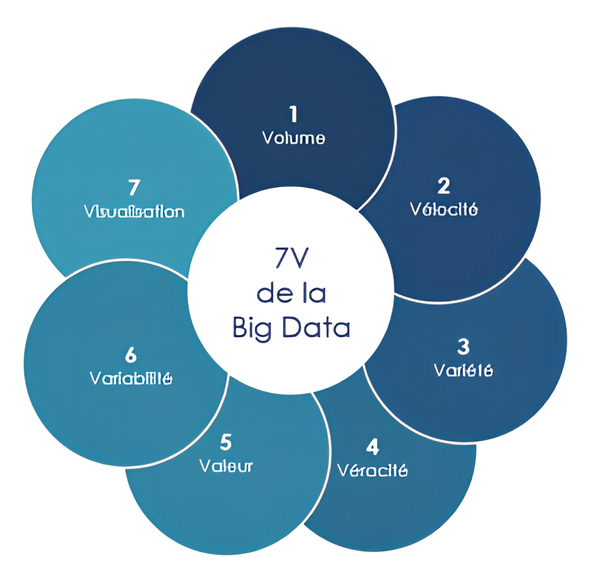
\includegraphics[width=0.55\textwidth]{images/7v.png}
    \caption{Les 7 V du Big Data}
    \label{fig:7v}
\end{figure}

\subsection{Enjeux spécifiques au projet}

Dans le contexte du triage automatique de tickets JIRA, le Big Data se manifeste à travers plusieurs enjeux concrets. Le premier est d'ordre volumétrique : le corpus Apache Spark totalise près de 50 000 tickets, chacun accompagné de commentaires, d'un journal de modifications et de relations inter-tickets, produisant plusieurs millions d'enregistrements à ingérer et transformer.

Le second enjeu est la variété des données. Les tickets combinent des données structurées (statut, priorité, dates, identifiants), des données semi-structurées (métadonnées JSON de l'API JIRA) et des données non structurées (descriptions textuelles, commentaires en langage naturel). Leur traitement conjoint exige une architecture unifiée capable de gérer ces formats hétérogènes.

Le troisième enjeu est celui de la qualité et de la véracité. Les descriptions de tickets varient considérablement en longueur, en langue (anglais, français, termes techniques mixtes) et en précision. Certains champs sont absents ou incohérents. Un processus de nettoyage et de normalisation rigoureux est indispensable pour alimenter un pipeline de classification fiable.

Enfin, la valeur produite doit être tangible et directement exploitable par les équipes opérationnelles : prédictions de catégorie, estimation de la résolution probable et résumés correctifs actionnables.

%------------------------2--------------------------
\section{Architectures de stockage et de traitement des données}

\subsection{Du Data Warehouse traditionnel au Cloud Data Warehouse}

Le concept d'entrepôt de données (Data Warehouse) remonte aux travaux fondateurs de William Inmon \cite{logo:inmon} et Ralph Kimball \cite{logo:kimball} dans les années 1990. Un entrepôt de données est un référentiel centralisé conçu pour le reporting et l'analyse, alimenté par des processus ETL (Extract, Transform, Load) qui transforment les données opérationnelles en structures optimisées pour la lecture. Les systèmes traditionnels tels qu'Oracle Exadata ou Teradata ont longtemps dominé ce marché, mais ils souffrent de limitations importantes face aux volumes du Big Data : coût élevé des licences, scalabilité limitée et rigidité architecturale.

L'avènement du cloud computing a profondément modifié ce paysage en permettant l'émergence de solutions élastiques, facturées à l'usage et capables de traiter des pétaoctets de données. Ces plateformes cloud modernes dissocient généralement le stockage du calcul, permettant de dimensionner chaque ressource indépendamment selon les besoins.

\subsection{Panorama des plateformes cloud modernes}

\paragraph{Snowflake}

Snowflake \cite{logo:snowflake} est une plateforme de données cloud conçue dès l'origine pour le cloud, sans héritage d'architecture on-premise. Son architecture tri-couche, illustrée en figure \ref{fig:snowflake_archi}, sépare les services cloud (méta-données, sécurité, authentification), le calcul (entrepôts virtuels indépendants) et le stockage (S3, Azure Blob, GCS selon le cloud hôte). Cette séparation confère à Snowflake une élasticité remarquable : il est possible d'exécuter plusieurs charges de travail simultanément sur les mêmes données sans contention de ressources.

Snowflake prend nativement en charge le SQL ANSI, les données semi-structurées au format JSON (via le type \texttt{VARIANT}), le clonage instantané de tables sans duplication de données, et le partage sécurisé de données entre organisations. Sa couche d'intelligence artificielle intégrée, Snowflake Cortex, est détaillée dans la section~\ref{sec:cortex}.

\begin{figure}[H]
\centering
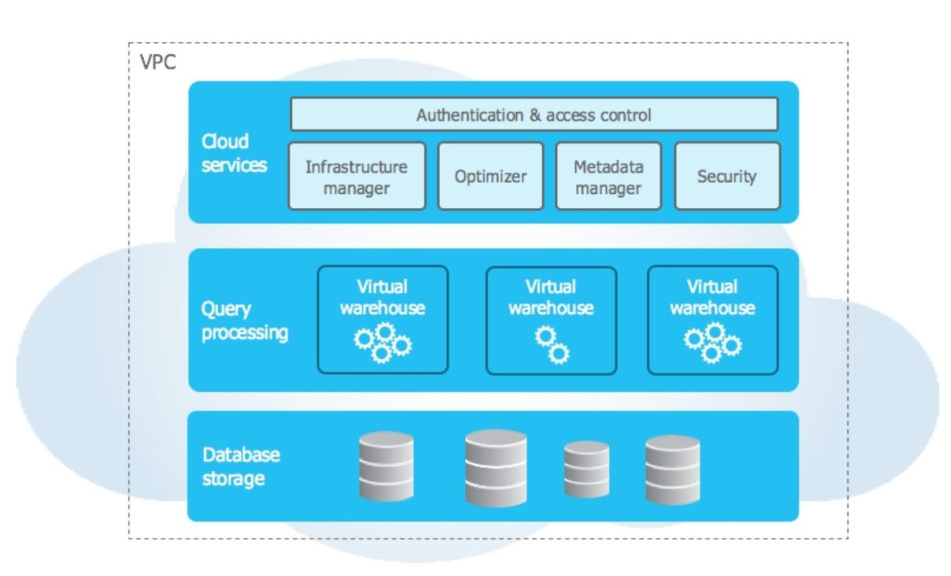
\includegraphics[width=0.85\textwidth]{images/archisnwoflake.png}
\caption{Architecture de Snowflake : séparation stockage, calcul et services}
\label{fig:snowflake_archi}
\end{figure}

\paragraph{Google BigQuery}

Google BigQuery \cite{logo:bigquery} est l'entrepôt de données serverless de Google Cloud Platform. Il repose sur le moteur de traitement Dremel, qui découpe automatiquement les requêtes en tâches parallèles exécutées sur des milliers de nœuds. BigQuery stocke les données en format colonne compressé sur le système de fichiers Colossus de Google, garantissant des performances élevées sur les requêtes analytiques portant sur de grandes plages temporelles. Il intègre BigQuery ML pour l'entraînement et l'inférence de modèles directement depuis SQL, ainsi que des connecteurs natifs vers les services d'IA de Google (Vertex AI \cite{logo:vertex_ai}).

\paragraph{Amazon Redshift}

Amazon Redshift \cite{logo:redshift} est le service d'entrepôt de données managé d'AWS. Il repose sur une architecture MPP (Massively Parallel Processing) et stocke les données en colonnes compressées sur des nœuds de calcul. Redshift Spectrum permet d'interroger des données stockées sur S3 sans les charger dans l'entrepôt. Redshift ML offre une intégration avec Amazon SageMaker pour l'entraînement automatique de modèles. Sa profonde intégration dans l'écosystème AWS en fait un choix naturel pour les organisations déjà investies dans cette infrastructure.

\paragraph{Azure Synapse Analytics}

Azure Synapse Analytics \cite{logo:synapse} est la solution unifiée de Microsoft combinant entrepôt de données analytiques et traitement Big Data. Il permet d'interroger indifféremment des données stockées dans Azure Data Lake Storage via SQL serverless ou dans des pools SQL dédiés. Son intégration avec Azure Machine Learning, Azure OpenAI Service et Power BI en fait une plateforme bout-en-bout pour les organisations de l'écosystème Microsoft.

\subsection{L'architecture Lakehouse}

L'architecture Lakehouse \cite{logo:databricks}, popularisée par Databricks, cherche à réunir les avantages complémentaires du data lake (stockage flexible et peu coûteux de données brutes dans des formats ouverts) et du data warehouse (performances analytiques, garanties transactionnelles, gouvernance). La figure \ref{fig:lakehouse_archi} illustre cette architecture hybride.

\begin{figure}[H]
\centering
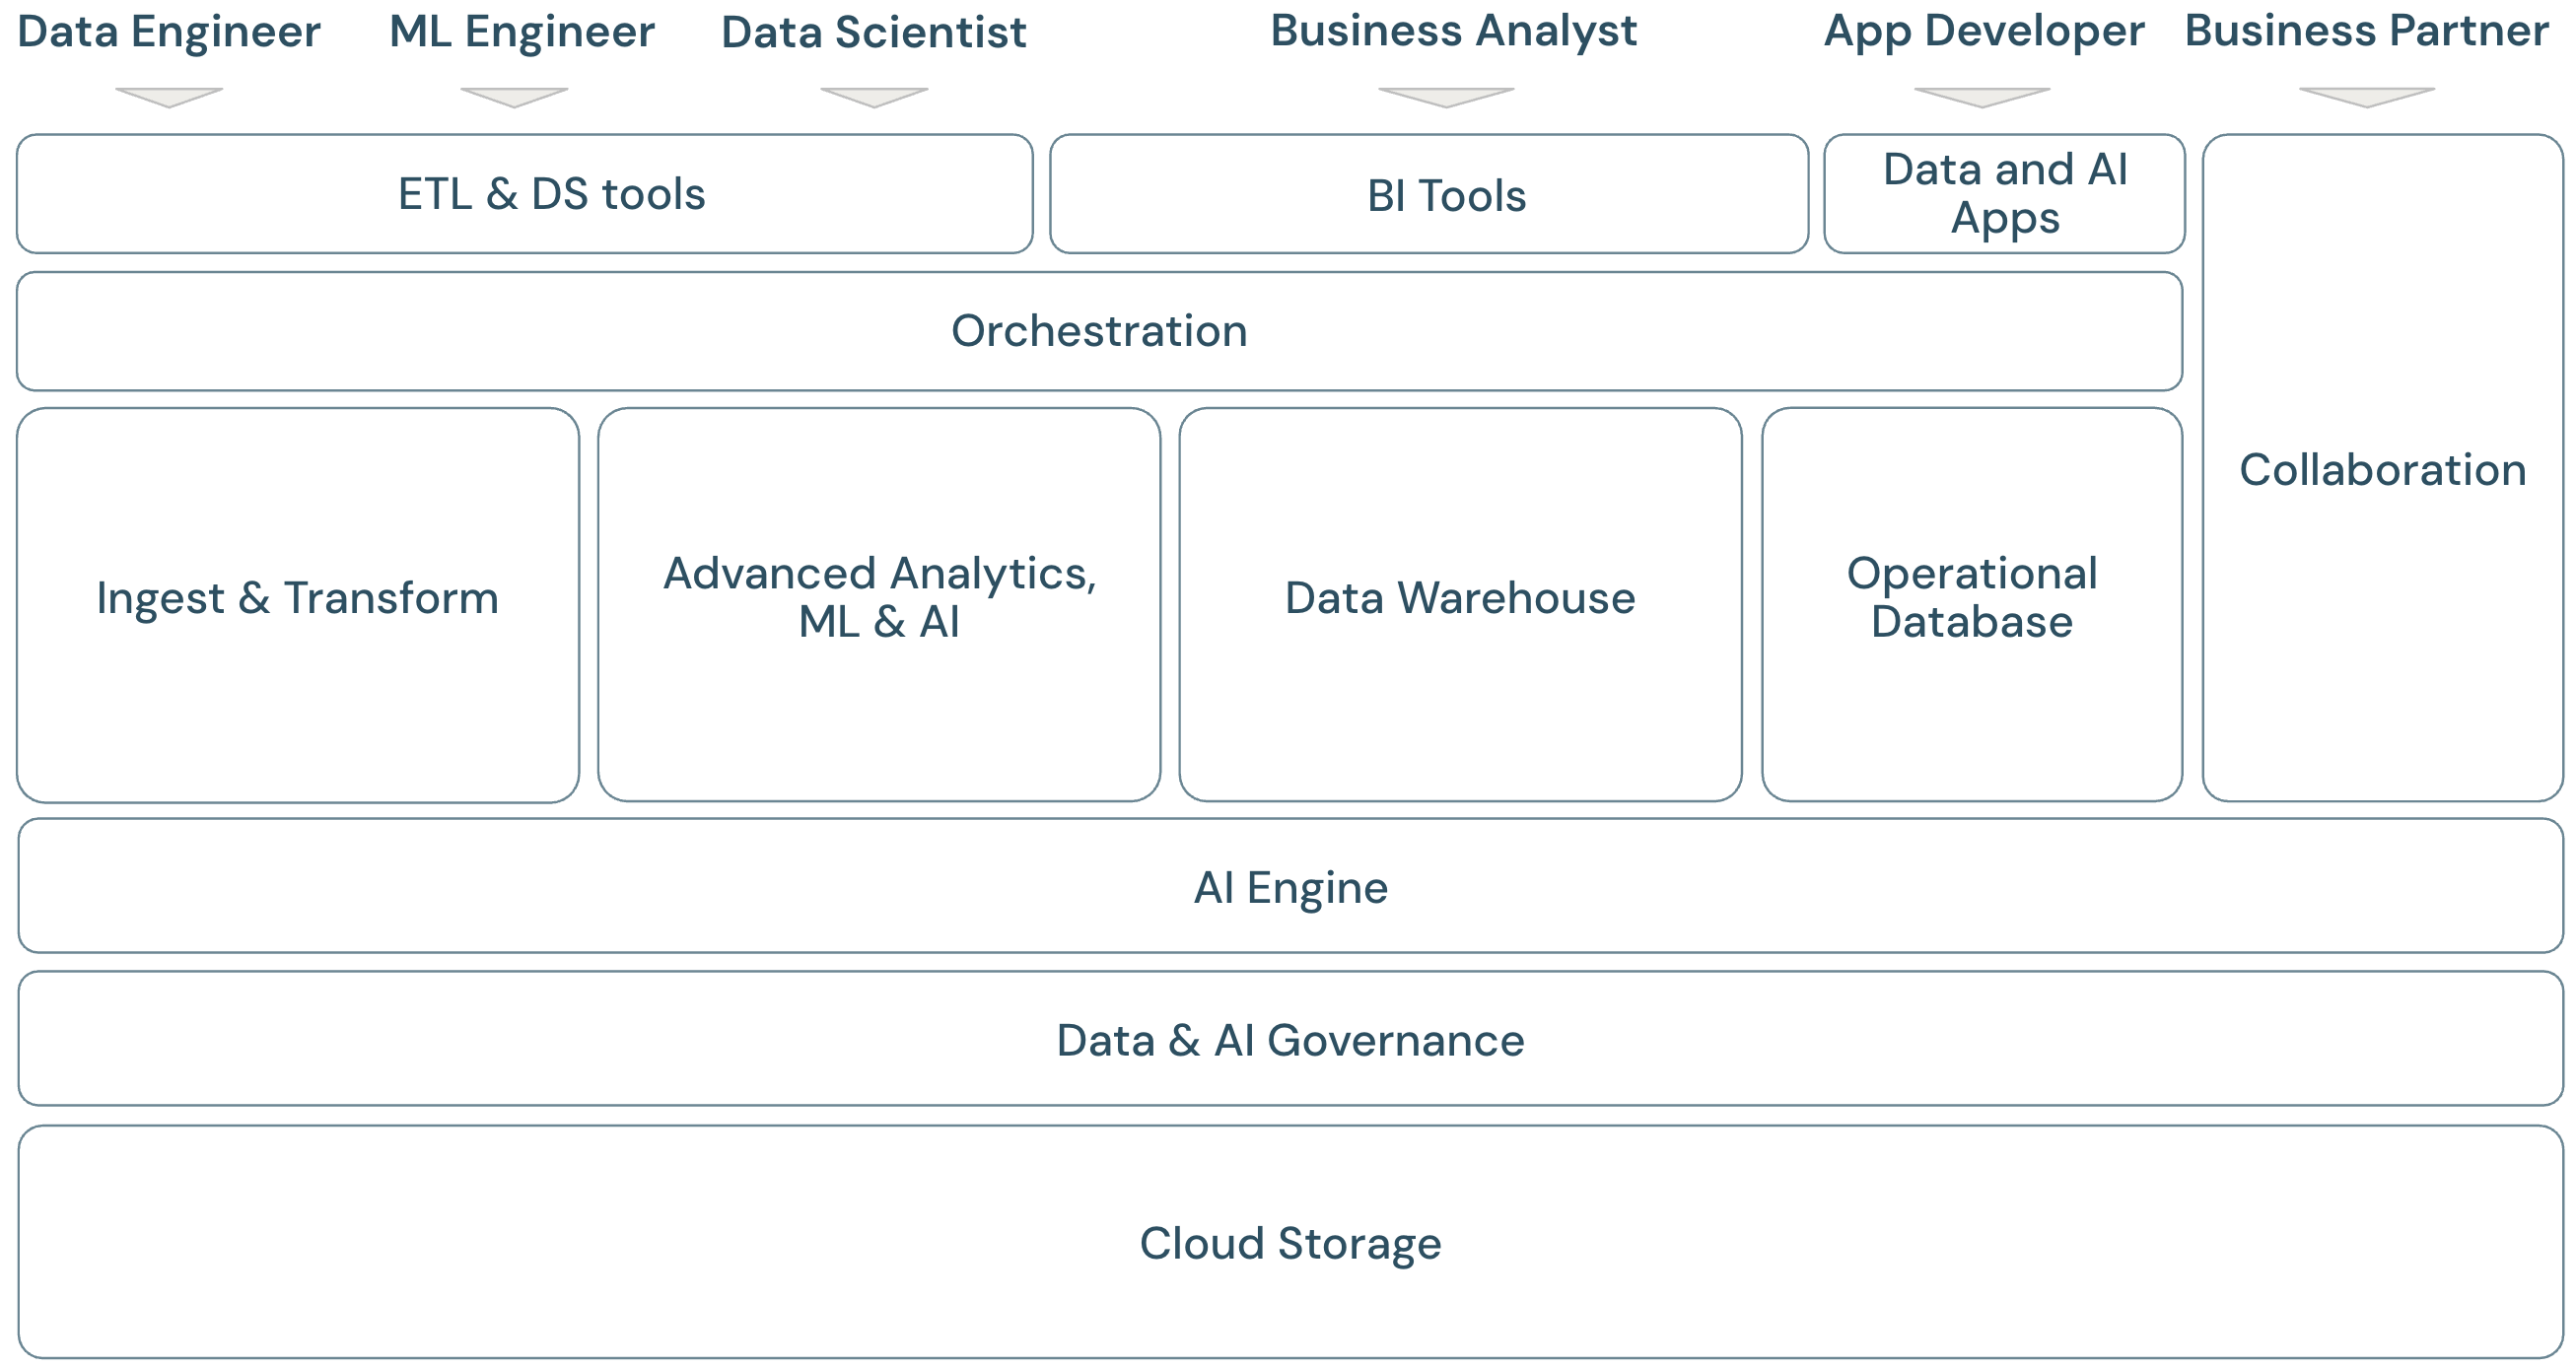
\includegraphics[width=0.85\textwidth]{images/lakehouse_architecture.png}
\caption{Architecture Lakehouse selon Databricks}
\label{fig:lakehouse_archi}
\end{figure}

Le format ouvert Delta Lake constitue la pierre angulaire de cette architecture : il ajoute une couche transactionnelle conforme aux propriétés ACID au-dessus de fichiers Parquet stockés dans un data lake. D'autres formats ouverts comme Apache Iceberg ou Apache Hudi répondent à des objectifs similaires et connaissent une adoption croissante. Databricks construit au-dessus de cette fondation une plateforme unifiée pour l'ingénierie des données (pipelines Spark), la data science et l'analyse SQL.

\subsection{Tableau comparatif des plateformes}

Le tableau \ref{tab:comparatif_dw} synthétise les caractéristiques des principales plateformes selon les critères pertinents pour notre projet.

\begin{table}[h!]
\centering
\begin{tabularx}{\textwidth}{|l|X|X|X|X|}
  \hline
  \textbf{Critère} & \textbf{Snowflake} & \textbf{BigQuery} & \textbf{Redshift} & \textbf{Databricks} \\
  \hline
  Modèle de facturation & Crédits (stockage + calcul séparés) & À la requête ou forfait & Instance réservée & DBU (unité de traitement) \\
  \hline
  Multi-cloud natif & Oui (AWS, GCP, Azure) & Non (GCP) & Non (AWS) & Oui \\
  \hline
  Formats semi-structurés & Natif (VARIANT) & Natif & Via Spectrum & Via Delta Lake \\
  \hline
  IA intégrée & Cortex (LLM, embeddings) & BigQuery ML, Vertex AI & SageMaker & MLflow, Model Serving \\
  \hline
  Architecture & Séparation calcul/stockage & Serverless & MPP & Lakehouse (Spark) \\
  \hline
  Conformité données & Élevée (données dans Snowflake) & GCP (certifications SOC2) & AWS (certifications SOC2) & Dépend du cloud hôte \\
  \hline
\end{tabularx}
\caption{Comparaison des principales plateformes de données cloud}
\label{tab:comparatif_dw}
\end{table}

%------------------------3--------------------------
\section{Outils de transformation et d'orchestration des données}

\subsection{Le paradigme ELT et les outils de transformation}

L'ingénierie des données repose traditionnellement sur le paradigme ETL (Extract, Transform, Load), où les transformations sont effectuées dans un moteur intermédiaire avant chargement dans l'entrepôt. L'avènement des entrepôts cloud puissants a favorisé l'émergence du paradigme ELT (Extract, Load, Transform), dans lequel les données brutes sont chargées dans l'entrepôt avant d'y être transformées en exploitant directement sa puissance de calcul. Cette inversion simplifie l'architecture et améliore les performances pour les transformations analytiques.

\paragraph{dbt (Data Build Tool)}

dbt \cite{logo:dbt} est l'outil de référence du paradigme ELT moderne. Il applique les principes du génie logiciel au travail de transformation de données : les modèles sont versionnés, testés, documentés et organisés en graphe acyclique dirigé (DAG) garantissant un ordre d'exécution correct et une reproductibilité totale. La figure \ref{fig:dbt_workflow} illustre le fonctionnement de dbt.

\begin{figure}[H]
\centering
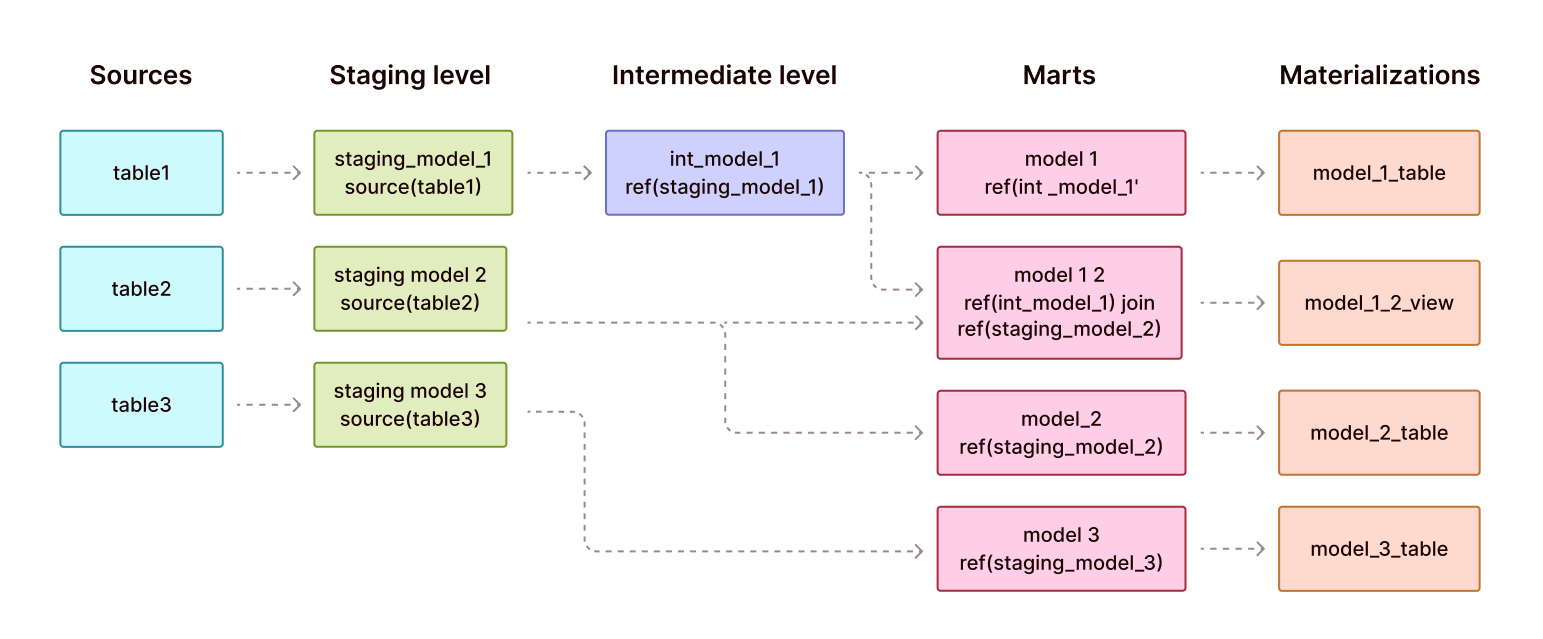
\includegraphics[width=0.85\textwidth]{images/dbt_workflow.png}
\caption{Fonctionnement de dbt : transformations SQL orchestrées dans l'entrepôt}
\label{fig:dbt_workflow}
\end{figure}

Chaque modèle dbt est un fichier SQL représentant une transformation. dbt génère le code d'exécution approprié (création de vues ou de tables matérialisées) et le soumet directement à l'entrepôt. Les tests intégrés permettent de valider automatiquement l'unicité des clés, l'absence de valeurs nulles inattendues, les plages de valeurs admissibles et les relations référentielles. La documentation est générée automatiquement à partir des modèles et des métadonnées associées.

\paragraph{Talend}

Talend \cite{logo:talend} est une plateforme d'intégration de données qui propose une approche ETL graphique. Ses composants préconfigurés permettent de concevoir des pipelines sans écrire de code, ce qui la rend accessible aux profils non développeurs. Talend dispose de nombreux connecteurs vers les sources de données hétérogènes. Cependant, sa complexité opérationnelle, son modèle de licence et ses performances sur de très grands volumes en font un outil moins adapté aux architectures ELT modernes.

\paragraph{Apache NiFi}

Apache NiFi \cite{logo:nifi} est une plateforme d'automatisation des flux de données, particulièrement adaptée à l'ingestion en temps réel depuis des sources hétérogènes. Son interface visuelle permet de construire des pipelines drag-and-drop, et son architecture distribuée assure une haute disponibilité. NiFi excelle pour l'ingestion et le routage de flux, mais ses capacités de transformation analytique restent limitées comparées aux outils ELT dédiés.

\subsection{L'orchestration des workflows de données}

L'orchestration désigne la planification, la surveillance et la gestion des dépendances entre les tâches composant un pipeline de données. Elle répond à la nécessité de gérer des workflows complexes avec des dépendances, des reprises sur erreur, des notifications et une observabilité complète.

\paragraph{Apache Airflow}

Apache Airflow \cite{logo:airflow} est l'orchestrateur de workflows open source le plus répandu dans l'écosystème de données. Les pipelines sont définis en Python sous forme de DAG, offrant une expressivité totale. Airflow dispose d'une interface web riche pour la surveillance et d'un écosystème important de connecteurs (opérateurs) vers les systèmes externes. La figure \ref{fig:airflow_dag} illustre un exemple de DAG dans Airflow.

\begin{figure}[H]
\centering
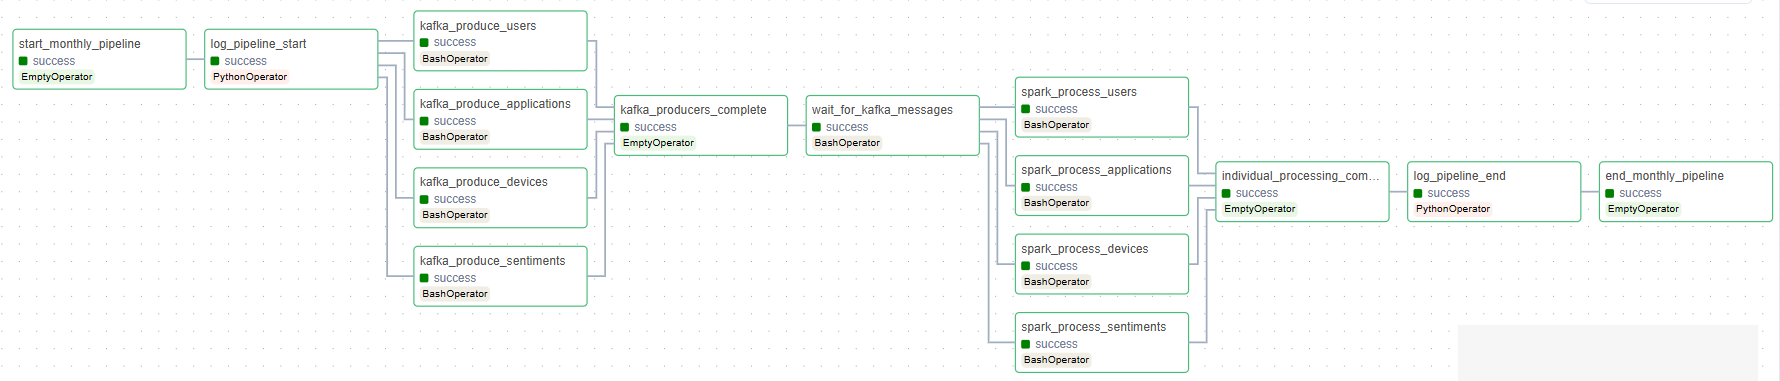
\includegraphics[width=0.85\textwidth]{images/airflow_dag.png}
\caption{Exemple de DAG dans Apache Airflow}
\label{fig:airflow_dag}
\end{figure}

\paragraph{Prefect et Dagster}

Prefect \cite{logo:prefect} et Dagster \cite{logo:dagster} sont des orchestrateurs de nouvelle génération qui répondent à certaines limitations d'Airflow. Prefect met l'accent sur la résilience et la testabilité des workflows, avec une approche orientée flux de données. Dagster introduit le concept d'asset software-defined, où l'orchestration est centrée non plus sur les tâches mais sur les données produites, facilitant la traçabilité et la gestion des dépendances dans les grands projets de données.

\subsection{Tableau comparatif des outils de transformation et d'orchestration}

\begin{table}[h!]
\centering
\begin{tabularx}{\textwidth}{|l|X|X|X|}
  \hline
  \textbf{Critère} & \textbf{dbt} & \textbf{Talend} & \textbf{Apache NiFi} \\
  \hline
  Paradigme & ELT (SQL dans l'entrepôt) & ETL (moteur externe) & Ingestion/flux \\
  \hline
  Courbe d'apprentissage & Faible (SQL) & Moyenne (interface graphique) & Moyenne \\
  \hline
  Tests et qualité & Intégrés nativement & Partiels & Limités \\
  \hline
  Documentation auto & Oui (DAG interactif) & Partielle & Non \\
  \hline
  Adapté à ELT cloud & Oui & Non & Non \\
  \hline
  Open source & Oui (Core) & Partiellement & Oui \\
  \hline
\end{tabularx}
\caption{Comparaison des outils de transformation de données}
\label{tab:comparatif_transformation}
\end{table}

%------------------------4--------------------------
\section{Intelligence artificielle appliquée au traitement du texte}

\subsection{Évolution du traitement automatique du langage naturel}

Le traitement automatique du langage naturel (TALN, ou NLP en anglais) est la discipline de l'intelligence artificielle qui s'intéresse à la compréhension et à la génération du langage humain par les machines. Appliqué à la classification de tickets logiciels, le NLP permet d'analyser automatiquement le contenu textuel des descriptions d'incidents pour en inférer la catégorie, la priorité et la résolution probable.

\subsubsection{Approches classiques : représentations vectorielles creuses}

Les premières approches de classification de texte reposaient sur des représentations vectorielles creuses. Le modèle sac-de-mots (bag-of-words) représente chaque document comme un vecteur dont les composantes correspondent aux fréquences des termes du vocabulaire, indépendamment de leur ordre d'apparition. La pondération TF-IDF (Term Frequency–Inverse Document Frequency) \cite{logo:tfidf} raffine cette représentation en diminuant le poids des termes fréquents dans l'ensemble du corpus (déterminants, verbes courants) et en valorisant les termes discriminants.

Ces représentations alimentent des classifieurs statistiques éprouvés : machines à vecteurs de support (SVM), forêts aléatoires (Random Forests), régression logistique, classifieurs naïfs de Bayes. Ces méthodes ont produit des résultats satisfaisants sur les corpus de petite taille et les tâches simples. Cependant, elles souffrent de deux limitations fondamentales : elles ne capturent pas la sémantique des termes (deux mots synonymes sont traités comme distincts), et la haute dimensionnalité des vecteurs creuses pose des problèmes de généralisation et de complexité computationnelle.

\subsubsection{Représentations distribuées : l'ère des word embeddings}

L'introduction des représentations distribuées a constitué une rupture paradigmatique dans le TALN. L'idée fondatrice, issue de l'hypothèse distributionnelle de Harris (1954), est que le sens d'un mot peut être inféré de son contexte d'apparition. Des mots apparaissant dans des contextes similaires ont des représentations vectorielles proches dans l'espace d'embedding.

\paragraph{Word2Vec}

Word2Vec \cite{logo:word2vec}, proposé par Mikolov et al. (2013) chez Google, est le premier modèle d'embedding à grande échelle à démontrer l'utilité pratique des représentations distribuées. Il repose sur deux architectures d'entraînement complémentaires : le modèle CBOW (Continuous Bag-of-Words), qui prédit un mot à partir des mots de son contexte, et le modèle Skip-gram, qui prédit les mots du contexte à partir du mot central. Word2Vec produit des représentations vectorielles denses de quelques centaines de dimensions qui capturent des analogies sémantiques remarquables.

La principale limite de Word2Vec est son caractère statique : chaque mot reçoit un vecteur unique, quelle que soit sa polysémie. Le terme \textit{« banque »} possède le même vecteur qu'il désigne un établissement financier ou la rive d'un cours d'eau.

\paragraph{GloVe}

GloVe (Global Vectors for Word Representation) \cite{logo:glove}, proposé par Pennington et al. (2014) à Stanford, adopte une approche différente : il factorise la matrice de co-occurrence globale du corpus pour produire des embeddings capturant à la fois les statistiques locales et globales du langage. GloVe offre des performances comparables à Word2Vec sur de nombreuses tâches, avec un entraînement plus efficace sur de grands corpus.

\paragraph{ELMo}

ELMo (Embeddings from Language Models) \cite{logo:elmo}, proposé par Peters et al. (2018), introduit des représentations contextuelles au niveau du mot. Le vecteur d'un terme est calculé dynamiquement en fonction de son contexte phrastique, résolvant ainsi le problème de polysémie. ELMo repose sur des réseaux récurrents LSTM bidirectionnels pré-entraînés sur de larges corpus textuels.

\subsubsection{La révolution Transformer}

L'architecture Transformer \cite{logo:transformer}, proposée par Vaswani et al. en 2017 dans l'article fondateur \textit{Attention is All You Need}, a profondément transformé le domaine du TALN et au-delà. Son mécanisme central, l'auto-attention (self-attention), permet au modèle de pondérer dynamiquement l'importance de chaque élément d'une séquence par rapport à tous les autres éléments, capturant ainsi les dépendances à longue portée sans les limitations des architectures récurrentes.

À la différence des réseaux de neurones récurrents (RNN, LSTM), qui traitent les séquences de manière séquentielle et peinent à propager l'information sur de longues distances, le Transformer traite tous les éléments de la séquence en parallèle. Cela permet un entraînement plus efficace sur des corpus massifs et une meilleure capture des dépendances sémantiques complexes.

Le mécanisme d'attention multi-têtes permet au modèle de capturer simultanément différents types de relations entre les tokens (relations syntaxiques, coréférentielles, sémantiques), en calculant l'attention selon plusieurs sous-espaces de représentation indépendants dont les résultats sont ensuite concaténés.

\subsection{Les modèles pré-entraînés et le paradigme du transfert d'apprentissage}

\subsubsection{BERT et ses dérivés}

BERT (Bidirectional Encoder Representations from Transformers) \cite{logo:bert}, proposé par Devlin et al. (2018) chez Google, a inauguré l'ère des modèles de langage pré-entraînés à grande échelle. BERT est un encodeur Transformer bidirectionnel pré-entraîné sur deux tâches non supervisées : la prédiction de mots masqués (Masked Language Modeling) et la prédiction de la relation entre deux phrases consécutives (Next Sentence Prediction). Ce pré-entraînement sur de vastes corpus (BooksCorpus et Wikipedia anglaise) lui confère une représentation riche et généraliste du langage.

L'apport majeur de BERT est le paradigme pré-entraînement/fine-tuning : un modèle BERT pré-entraîné peut être adapté à une tâche spécifique (classification, extraction d'entités, question-réponse) en ajoutant une couche de prédiction et en réentraînant l'ensemble sur un petit corpus annoté. Cette approche a établi de nouveaux records de performance sur la quasi-totalité des benchmarks NLP de l'époque.

De nombreux modèles dérivés ont suivi : RoBERTa \cite{logo:roberta} (Meta, entraînement optimisé avec davantage de données), DistilBERT (modèle allégé par distillation de connaissance), CamemBERT pour le français, DeBERTa (Microsoft, mécanisme d'attention décorrelé). Chacun apporte des améliorations sur des aspects spécifiques tout en conservant l'architecture encodeur bidirectionnelle de BERT.

\subsubsection{Les modèles d'embedding de phrases}

La classification de tickets requiert non pas des embeddings au niveau du mot, mais des représentations vectorielles de phrases ou de paragraphes entiers. La bibliothèque \texttt{sentence-transformers} \cite{logo:sentence_transformers}, proposée par Reimers et Gurevych (2019), adapte les modèles BERT à cette tâche via un entraînement par paires de phrases similaires et dissimilaires (apprentissage contrastif siamois). Ce paradigme d'entraînement assure que des phrases sémantiquement proches produisent des embeddings proches dans l'espace vectoriel.

Parmi les modèles d'embedding de référence, on distingue :
\begin{itemize}
    \item \textbf{all-MiniLM-L6-v2 \cite{logo:sentence_transformers} :} Un modèle compact offrant un bon équilibre entre qualité des embeddings (384 dimensions) et vitesse d'inférence sur CPU. Particulièrement adapté aux environnements contraints en ressources computationnelles.
    \item \textbf{E5 (Microsoft) \cite{logo:e5} :} Une famille de modèles optimisés pour la recherche sémantique et le reranking, entraînés sur de vastes corpus de paires textuelles.
    \item \textbf{voyage-multilingual-2 (Voyage AI) \cite{logo:snowflake_cortex} :} Un modèle multilingue de haute performance couvrant plus de 30 langues, particulièrement adapté aux corpus techniques comportant des termes issus de plusieurs langues.
    \item \textbf{text-embedding-3-large (OpenAI) \cite{logo:openai} :} Un modèle propriétaire accessible via API, produisant des vecteurs de 3072 dimensions avec des performances de pointe sur les benchmarks MTEB.
\end{itemize}

\subsection{Les grands modèles de langage}

\subsubsection{Définition et principes fondamentaux}

Les grands modèles de langage (LLM, Large Language Models) sont des modèles Transformer pré-entraînés sur des corpus textuels massifs comptant des centaines de milliards de tokens, avec des paramètres se chiffrant en milliards. Leur pré-entraînement via des objectifs auto-supervisés (modélisation du langage causal ou masqué) leur confère une connaissance généraliste du langage et du monde, exploitable sans réentraînement par simple formulation de la tâche dans un prompt : c'est le principe du zero-shot et du few-shot learning.

Les LLM modernes surpassent les approches précédentes sur une vaste gamme de tâches : compréhension de texte, génération de contenu structuré, raisonnement, extraction d'informations, traduction, résumé et classification. Leur capacité à traiter des fenêtres de contexte de plus en plus larges (jusqu'à plusieurs centaines de milliers de tokens pour les modèles récents) leur permet d'intégrer des instructions détaillées et des exemples directement dans le prompt.

\subsubsection{Panorama des principales familles de LLM}

\paragraph{La famille GPT (OpenAI)}

La série GPT (Generative Pre-trained Transformer) \cite{logo:openai} représente l'évolution la plus emblématique des modèles auto-régressifs génératifs. GPT-3 (2020) a démontré pour la première fois les capacités de few-shot learning à grande échelle. GPT-4 et ses déclinaisons (GPT-4o, GPT-4 Turbo) ont ensuite établi de nouveaux standards en matière de raisonnement, de compréhension contextuelle et de génération de code. Ces modèles sont accessibles via l'API OpenAI et sont particulièrement performants pour les tâches de génération de contenu structuré et de raisonnement complexe.

\paragraph{La famille Claude (Anthropic)}

La famille Claude \cite{logo:anthropic_api} est développée par Anthropic selon des principes d'alignement rigoureux. Claude se distingue par sa fenêtre de contexte étendue (jusqu'à 200 000 tokens pour Claude 3 Opus), sa précision sur les tâches d'analyse de texte long, et son orientation vers la sécurité et la fiabilité des sorties. La conception de ces modèles intègre des techniques d'apprentissage par renforcement à partir du retour humain (RLHF) et d'apprentissage constitutionnel (Constitutional AI), réduisant les sorties nuisibles ou inappropriées.

\paragraph{La famille Llama (Meta)}

Meta AI propose avec la famille Llama \cite{logo:llama} des modèles à poids ouverts (open weights), permettant un déploiement local ou dans des environnements cloud maîtrisés sans transmission de données vers des tiers. Llama 3, avec ses variantes de 8B et 70B paramètres, offre des performances comparables aux modèles propriétaires sur de nombreuses tâches de compréhension et de génération, tout en préservant la confidentialité des données sensibles.

\paragraph{La famille Mistral}

Mistral AI, société française fondée en 2023, a rapidement acquis une réputation d'excellence dans le domaine des LLM efficaces. Le modèle Mistral 7B \cite{logo:mistral} a démontré que des modèles de taille modérée, entraînés avec soin, peuvent rivaliser avec des modèles bien plus grands. Mistral Large 2 est particulièrement reconnu pour son rapport performances/coût favorable et ses capacités en contexte multilingue. Son architecture intègre des mécanismes d'attention à fenêtre glissante (sliding window attention) et de regroupement de têtes d'attention (grouped-query attention) qui optimisent l'efficacité computationnelle.

\subsubsection{Stratégies d'utilisation des LLM}

Plusieurs stratégies permettent d'exploiter les LLM selon les contraintes et les objectifs du projet :

\begin{itemize}
    \item \textbf{Zero-shot prompting :} Le modèle est sollicité directement sur la tâche sans exemple préalable. Cette approche exploite la connaissance générale acquise lors du pré-entraînement. Elle est simple à mettre en œuvre mais peut manquer de précision sur des tâches très spécifiques à un domaine.

    \item \textbf{Few-shot prompting :} Quelques exemples représentatifs de la tâche sont fournis dans le prompt pour guider le modèle. Les exemples agissent comme des démonstrations in-context qui orientent le format et le contenu de la réponse. Cette approche améliore significativement la précision sans nécessiter de réentraînement.

    \item \textbf{Chain-of-thought prompting :} Le modèle est invité à détailler son raisonnement étape par étape avant de formuler sa réponse. Cette technique, proposée par Wei et al. \cite{logo:cot}, améliore les performances sur les tâches requérant un raisonnement multi-étapes, au prix d'une latence et d'un coût en tokens plus élevés.

    \item \textbf{Fine-tuning supervisé :} Le modèle pré-entraîné est réentraîné sur un corpus annoté spécifique à la tâche. Cette approche offre les meilleures performances sur le domaine cible, mais nécessite des données annotées de qualité, une infrastructure GPU dédiée et une expertise en entraînement de modèles.

    \item \textbf{Retrieval-Augmented Generation (RAG) :} Le modèle est enrichi dynamiquement avec des informations pertinentes récupérées depuis une base de connaissances externe au moment de l'inférence. Cette approche est détaillée dans la section suivante.
\end{itemize}

%------------------------5--------------------------
\section{La recherche sémantique et les bases de données vectorielles}

\subsection{Principe de la recherche vectorielle}

La recherche vectorielle repose sur la représentation des documents sous forme de vecteurs denses dans un espace de haute dimension, puis sur l'identification des vecteurs les plus proches d'une requête selon une mesure de similarité donnée. Contrairement à la recherche par mots-clés (qui requiert une correspondance exacte de termes), la recherche vectorielle capture la proximité sémantique : deux textes exprimant la même idée avec des termes différents se retrouvent proches dans l'espace d'embedding.

\subsection{Mesures de similarité vectorielle}

Le choix de la mesure de similarité influe sur la qualité des résultats de recherche. Les trois mesures les plus utilisées sont :

\begin{itemize}
    \item \textbf{Similarité cosinus :} Mesure l'angle entre deux vecteurs, indépendamment de leur norme. C'est la mesure de référence pour les embeddings de texte, car elle est invariante à la longueur du document. Elle retourne une valeur entre $-1$ et $1$, où $1$ indique une orientation identique dans l'espace vectoriel.

    \item \textbf{Distance euclidienne (L2) :} Mesure la distance géométrique entre deux points dans l'espace vectoriel. Contrairement à la similarité cosinus, elle est sensible à la norme des vecteurs et peut être affectée par les variations de longueur des textes.

    \item \textbf{Produit scalaire (inner product) :} Prend en compte à la fois l'angle et la magnitude des vecteurs. Utilisé lorsque la norme du vecteur encode une information de pertinence, notamment dans certains systèmes de recommandation.
\end{itemize}

La recherche des $k$ plus proches voisins ($k$-NN) consiste à retrouver, parmi un corpus de référence préalablement indexé, les $k$ vecteurs les plus similaires à un vecteur requête. Pour les corpus de grande taille, des algorithmes d'indexation approximative (Approximate Nearest Neighbor, ANN), tels que HNSW (Hierarchical Navigable Small World) \cite{logo:hnsw} ou FAISS (Facebook AI Similarity Search) \cite{logo:faiss}, permettent d'effectuer cette recherche en temps sous-linéaire avec un compromis acceptable sur la précision.

\subsection{Bases de données vectorielles}

L'essor des LLM et des applications de recherche sémantique a favorisé l'émergence d'une nouvelle catégorie de systèmes de gestion de données : les bases de données vectorielles \cite{logo:vector_db_survey}. Ces systèmes sont optimisés pour le stockage, l'indexation et la recherche efficace de vecteurs denses à haute dimension. Le tableau \ref{tab:vector_db} présente les principales solutions disponibles.

\begin{table}[h!]
\centering
\begin{tabularx}{\textwidth}{|l|X|X|X|}
  \hline
  \textbf{Solution} & \textbf{Type} & \textbf{Points forts} & \textbf{Limitations} \\
  \hline
  Pinecone \cite{logo:pinecone} & Service managé (cloud) & Facilité d'utilisation, scalabilité, faible latence & Coût élevé, dépendance fournisseur \\
  \hline
  Weaviate \cite{logo:weaviate} & Open source / cloud & Multimodal, GraphQL, modules IA & Complexité de déploiement \\
  \hline
  Chroma \cite{logo:chroma} & Open source (local) & Légèreté, intégration LangChain & Scalabilité limitée \\
  \hline
  pgvector \cite{logo:pgvector} & Extension PostgreSQL & Intégration SQL native, pas d'infra supplémentaire & Performances ANN limitées \\
  \hline
  Snowflake Cortex \cite{logo:snowflake_cortex} & Intégré à Snowflake & Aucune extraction de données, SQL natif & Ecosystème Snowflake uniquement \\
  \hline
  Qdrant \cite{logo:qdrant} & Open source / cloud & Haute performance, filtrage riche & Moins mature que Pinecone \\
  \hline
\end{tabularx}
\caption{Comparaison des bases de données vectorielles}
\label{tab:vector_db}
\end{table}

%------------------------6--------------------------
\section{Le paradigme RAG (Retrieval-Augmented Generation)}

\subsection{Motivation et principes}

Le paradigme RAG \cite{logo:rag}, introduit par Lewis et al. (2020) chez Facebook AI Research, répond à une limitation fondamentale des LLM : leur connaissance est figée au moment de l'entraînement et ne reflète pas les données spécifiques à un domaine ou à une organisation. Un LLM interrogé sur des incidents internes ou sur des connaissances très spécialisées risque de produire des réponses inventées (phénomène dit d'hallucination) car il n'a jamais été exposé à ces informations.

L'idée centrale du RAG est d'enrichir dynamiquement le prompt du modèle avec des documents pertinents récupérés depuis une base de connaissances externe au moment de l'inférence. Le modèle dispose ainsi d'un contexte factuel sur lequel appuyer sa réponse, réduisant drastiquement le risque d'hallucination et permettant une adaptation au domaine sans réentraînement.

\subsection{Architecture générale du RAG}

Un pipeline RAG s'articule autour de trois composantes principales :

\begin{enumerate}
    \item \textbf{Phase d'indexation (offline) :} Les documents de la base de référence sont encodés sous forme d'embeddings vectoriels et stockés dans une base de données vectorielle. Cette phase est exécutée une fois lors de l'initialisation du système, puis incrémentalement à chaque ajout de nouveaux documents.

    \item \textbf{Phase de récupération (online) :} Lorsqu'une requête arrive, elle est encodée par le même modèle d'embedding que celui utilisé lors de l'indexation. Les $k$ documents dont les vecteurs sont les plus proches du vecteur requête sont récupérés depuis la base vectorielle.

    \item \textbf{Phase de génération (online) :} Le LLM reçoit un prompt enrichi comprenant la requête originale et les documents récupérés, qu'il utilise comme contexte pour formuler sa réponse. La réponse est ainsi ancrée sur des faits concrets plutôt que sur les seules connaissances internes du modèle.
\end{enumerate}

\subsection{Variantes et évolutions du RAG}

La recherche a produit plusieurs variantes du RAG original qui améliorent ses performances selon des axes différents \cite{logo:advanced_rag} :

\begin{itemize}
    \item \textbf{RAG naïf :} L'implémentation basique décrite ci-dessus. Efficace pour des cas simples mais sensible à la qualité des documents récupérés.

    \item \textbf{RAG avancé (Advanced RAG) :} Intègre des étapes de pré-récupération (reformulation de la requête, décomposition en sous-questions) et de post-récupération (reranking des documents, filtrage par pertinence) pour améliorer la qualité du contexte fourni au LLM.

    \item \textbf{RAG modulaire :} Architecture plus flexible permettant d'échanger indépendamment les composantes d'indexation, de récupération et de génération, facilitant l'expérimentation et l'optimisation de chaque partie.

    \item \textbf{RAG hybride :} Combine la recherche vectorielle sémantique avec une recherche par mots-clés (BM25 ou similaire) pour bénéficier des avantages complémentaires des deux approches. La recherche sémantique capture la proximité de sens, tandis que la recherche lexicale capture les correspondances de termes techniques exacts.

    \item \textbf{GraphRAG (Microsoft) \cite{logo:graphrag} :} Enrichit la récupération avec des relations extraites sous forme de graphe de connaissance, permettant des raisonnements multi-sauts sur des informations reliées.
\end{itemize}

\subsection{RAG versus fine-tuning : analyse comparative}

Le choix entre RAG et fine-tuning est une décision architecturale fondamentale dans les projets d'IA appliquée. Le tableau \ref{tab:rag_vs_finetune} met en regard les deux approches selon les critères pertinents pour notre contexte.

\begin{table}[h!]
\centering
\begin{tabularx}{\textwidth}{|l|X|X|}
  \hline
  \textbf{Critère} & \textbf{RAG} & \textbf{Fine-tuning} \\
  \hline
  Données annotées requises & Non (documents non étiquetés suffisent) & Oui (paires entrée/sortie annotées) \\
  \hline
  Mise à jour des connaissances & Immédiate (ajout de documents) & Nécessite un réentraînement \\
  \hline
  Traçabilité des réponses & Élevée (sources identifiables) & Faible (connaissance internalisée) \\
  \hline
  Infrastructure requise & Base vectorielle + API LLM & GPU dédiés pour l'entraînement \\
  \hline
  Hallucinations & Réduites (ancrage factuel) & Persistantes si données insuffisantes \\
  \hline
  Coût de déploiement & Faible à moyen & Élevé (coût GPU) \\
  \hline
  Adaptation au domaine & Bonne & Excellente \\
  \hline
  Confidentialité des données & Élevée si base locale & Données exposées lors de l'entraînement \\
  \hline
\end{tabularx}
\caption{Comparaison des approches RAG et fine-tuning}
\label{tab:rag_vs_finetune}
\end{table}

%------------------------7--------------------------
\section{Classification automatique de tickets : état des travaux}

\subsection{Approches classiques de classification de tickets}

La classification automatique de tickets logiciels est un problème étudié depuis les années 2000 dans la communauté du génie logiciel. Les premières études ont appliqué les méthodes standard de classification de texte à ce problème, avec des résultats contrastés.

Antoniol et al. \cite{logo:antoniol2008} ont montré que les algorithmes de classification automatique pouvaient distinguer les rapports de bogues des demandes de nouvelles fonctionnalités avec une précision dépassant 80\%, en utilisant des représentations TF-IDF couplées à des classifieurs SVM ou naïfs de Bayes. Lamkanfi et al. \cite{logo:lamkanfi2010} ont étendu ces travaux en montrant que la prédiction de la sévérité des bogues atteignait des performances acceptables sur des projets open source bien documentés.

Ces approches classiques présentent cependant des limites bien documentées : sensibilité aux données déséquilibrées (certaines catégories étant rares), difficulté à gérer la variabilité lexicale des descriptions techniques, et incapacité à exploiter le contexte sémantique des termes.

\subsection{Apports du deep learning et des modèles pré-entraînés}

L'avènement des modèles pré-entraînés a relancé l'intérêt pour la classification automatique de tickets. Kallis et al. \cite{logo:kallis2019} ont proposé Ticket Tagger, un système de classification automatique d'issues GitHub reposant sur des plongements de texte rapides (FastText), atteignant plus de 90\% de précision sur la distinction entre rapports de bogues et demandes de fonctionnalités.

Des approches plus récentes ont démontré que des modèles BERT fine-tunés sur des corpus de tickets GitHub surpassent significativement les méthodes classiques, avec des gains de F1-score de 10 à 20 points selon la tâche \cite{logo:bert_bug}. Des travaux ont également montré l'intérêt de combiner les informations textuelles avec les métadonnées structurelles et les relations entre tickets pour améliorer la classification des rapports ambigus.

\subsection{Approches basées sur les grands modèles de langage}

Des travaux plus récents explorent l'utilisation directe des LLM pour la classification de tickets. Kochhar et al. \cite{logo:kochhar2014} ont étudié la reclassification fine des rapports d'incidents, montrant que des descripteurs structurés permettent d'automatiser cette tâche de manière fiable. Les approches zero-shot et few-shot sur GPT-4 montrent des performances comparables au fine-tuning de BERT sur plusieurs benchmarks de classification d'issues, sans nécessiter de données annotées \cite{logo:llm_bug_report}.

L'approche RAG appliquée aux tickets a été explorée dans plusieurs travaux récents \cite{logo:advanced_rag}. Elle permet d'ancrer les prédictions sur des tickets historiques similaires, améliorant la cohérence et la traçabilité des classifications. Le recours à un mécanisme de seuil de confiance pour arbitrer entre la voie rapide (similarité directe) et l'appel au LLM est une optimisation permettant de concilier coût et qualité.

\subsection{Travaux spécifiques sur Apache Spark}

Le corpus JIRA d'Apache Spark a été étudié dans plusieurs travaux de recherche portant sur la prédiction du composant affecté, l'identification des tickets urgents ou la détection des régressions \cite{logo:jira_apache}. Ces études confirment la richesse du corpus (diversité des catégories, grande variabilité linguistique, présence de termes techniques spécialisés) et la difficulté de la tâche, notamment pour les tickets ayant une description courte ou ambiguë.

%------------------------8--------------------------
\section{Intégration de l'IA dans les entrepôts de données cloud}

\subsection{Snowflake Cortex}
\label{sec:cortex}

Snowflake Cortex \cite{logo:snowflake_cortex} est l'ensemble des fonctions d'intelligence artificielle intégrées nativement à Snowflake. Son positionnement au sein de la couche de services de Snowflake est illustré en figure \ref{fig:cortex}. Il permet d'exécuter des modèles de langage et de calculer des embeddings vectoriels directement depuis des requêtes SQL, sans extraction ni transfert des données vers des services externes. Cette intégration native présente plusieurs avantages majeurs : la conformité des données (elles ne quittent pas l'environnement sécurisé Snowflake), la facturation unifiée via les crédits Snowflake et la simplicité d'intégration dans les pipelines dbt.

\begin{figure}[H]
\centering
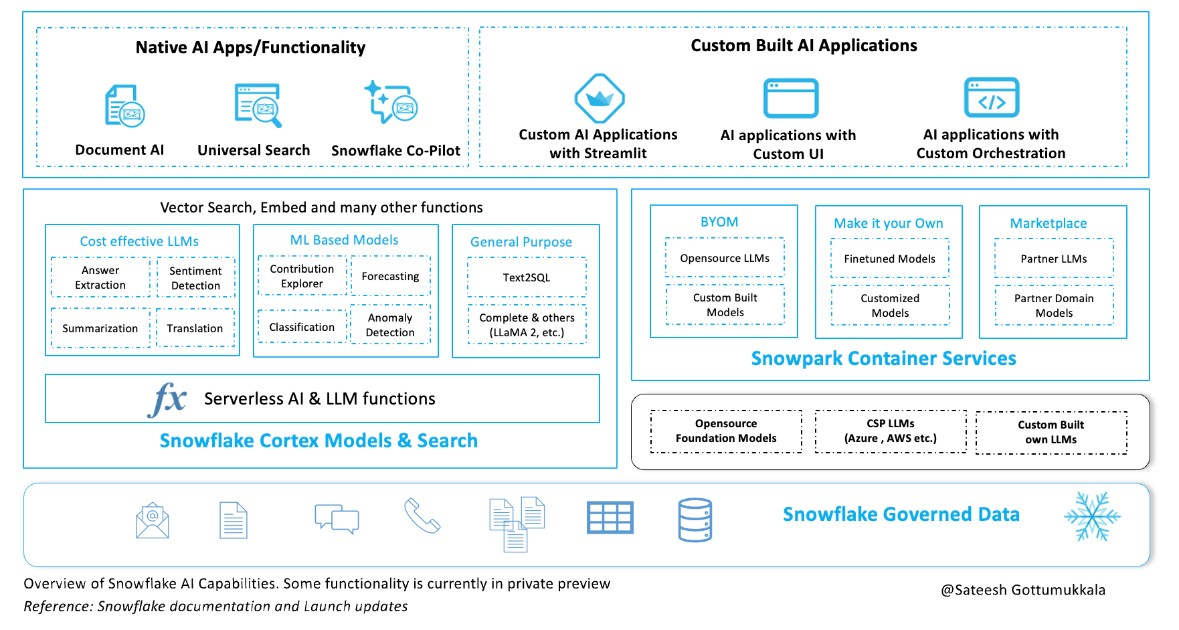
\includegraphics[width=0.85\textwidth]{images/cortexarchii.jpg}
\caption{Snowflake Cortex : fonctions IA intégrées à l'entrepôt de données}
\label{fig:cortex}
\end{figure}

Cortex propose un ensemble de fonctions couvrant les besoins courants en traitement du langage naturel : génération de texte par LLM (\texttt{CORTEX.COMPLETE}), calcul d'embeddings vectoriels (\texttt{CORTEX.EMBED\_TEXT}), résumé automatique (\texttt{CORTEX.SUMMARIZE}), traduction (\texttt{CORTEX.TRANSLATE}), analyse de sentiment (\texttt{CORTEX.SENTIMENT}), classification zero-shot (\texttt{CORTEX.CLASSIFY\_TEXT}) et extraction de réponses (\texttt{CORTEX.EXTRACT\_ANSWER}). Le tableau \ref{tab:cortex_fonctions} en présente les principales.

\begin{table}[h!]
\centering
\begin{tabularx}{\textwidth}{|l|X|X|}
  \hline
  \textbf{Fonction} & \textbf{Description} & \textbf{Cas d'usage typique} \\
  \hline
  \texttt{CORTEX.COMPLETE()} & Génération de texte par LLM. Supporte les modèles \texttt{mistral-large2}, \texttt{llama3.1-70b}, \texttt{llama3.1-8b}, \texttt{mixtral-8x7b}, etc. & Classification, extraction d'entités, génération de résumés structurés \\
  \hline
  \texttt{CORTEX.EMBED\_TEXT()} & Calcul du vecteur d'embedding d'un texte. Retourne un objet vectoriel natif. & Encodage de tickets, similarité sémantique, recherche $k$-NN \\
  \hline
  \texttt{CORTEX.SUMMARIZE()} & Génération d'un résumé concis d'un texte long. & Résumé de descriptions, synthèse de fils de discussion \\
  \hline
  \texttt{CORTEX.TRANSLATE()} & Traduction vers une langue cible (30+ langues). & Normalisation des tickets multilingues \\
  \hline
  \texttt{CORTEX.SENTIMENT()} & Analyse du sentiment, score continu entre $-1$ et $1$. & Priorisation par ton, détection d'insatisfaction \\
  \hline
  \texttt{CORTEX.CLASSIFY\_TEXT()} & Classification zero-shot sans entraînement préalable. & Triage de premier niveau \\
  \hline
  \texttt{CORTEX.EXTRACT\_ANSWER()} & Extraction de réponse à une question depuis un texte. & Extraction d'informations clés depuis une description d'incident \\
  \hline
\end{tabularx}
\caption{Fonctions LLM de Snowflake Cortex}
\label{tab:cortex_fonctions}
\end{table}

Snowflake Cortex intègre également un support natif des types vectoriels. Le type de données \texttt{VECTOR(FLOAT, n)} permet de stocker des vecteurs denses de dimension $n$, et des fonctions de similarité vectorielle (\texttt{VECTOR\_COSINE\_SIMILARITY}, \texttt{VECTOR\_L2\_DISTANCE}, \texttt{VECTOR\_INNER\_PRODUCT}) permettent d'implémenter la recherche des plus proches voisins directement en SQL, sans bibliothèque externe ni infrastructure dédiée.

\subsection{Comparaison des approches d'inférence LLM}

Trois grandes approches permettent d'intégrer des capacités LLM dans un pipeline de données. Le tableau \ref{tab:api_comparaison} en compare les caractéristiques essentielles.

\begin{table}[h!]
\centering
\begin{tabularx}{\textwidth}{|l|X|X|X|}
  \hline
  \textbf{Critère} & \textbf{Snowflake Cortex} & \textbf{APIs externes (OpenAI, Anthropic)} & \textbf{Bibliothèques locales (HuggingFace)} \\
  \hline
  Sortie de données & Non (données restent dans Snowflake) & Oui (envoi au fournisseur) & Non (tout local) \\
  \hline
  Taille des modèles & Grands modèles (70B+) & Très grands (GPT-4, Claude 3) & Limité par la RAM/GPU \\
  \hline
  Latence & Faible (réseau interne) & Variable (réseau public) & Faible (modèles légers) \\
  \hline
  Coût & Crédits Snowflake & Facturation à l'appel (tokens) & Gratuit (hors GPU) \\
  \hline
  Intégration SQL & Native & Non & Non \\
  \hline
  Conformité & Élevée & Dépend des CGU du fournisseur & Maximale \\
  \hline
\end{tabularx}
\caption{Comparaison des approches d'inférence LLM dans un pipeline de données}
\label{tab:api_comparaison}
\end{table}

\subsection{Autres plateformes intégrant l'IA}

Pour compléter l'analyse, notons que les autres grandes plateformes cloud proposent également des fonctionnalités d'IA intégrées. BigQuery ML \cite{logo:bigquery} permet d'entraîner des modèles classiques (régression, forêts aléatoires) directement depuis SQL et d'effectuer des inférences via des intégrations avec Vertex AI \cite{logo:vertex_ai}. Redshift ML \cite{logo:redshift} offre des fonctionnalités similaires via une intégration avec Amazon SageMaker AutoPilot. Databricks MLflow \cite{logo:mlflow} est un référentiel de gestion du cycle de vie des modèles (entraînement, versioning, déploiement) bien intégré dans l'écosystème Apache Spark et Delta Lake.

La différence structurante de Snowflake Cortex réside dans la disponibilité de LLM de grande taille (modèles à 70 milliards de paramètres et plus) directement accessibles depuis SQL, sans aucun déplacement des données, ce qui est déterminant dans un contexte de confidentialité et de gouvernance des données.

%------------------------9--------------------------
\section{Synthèse et justification des choix technologiques}

\subsection{Bilan comparatif global}

L'analyse des travaux existants et des technologies disponibles permet de dessiner les contours d'une architecture optimale pour notre projet. Plusieurs constats émergent de cette revue de littérature :

Premièrement, les approches classiques de classification de tickets (TF-IDF + SVM) atteignent rapidement leurs limites sur des corpus de grande taille avec une forte variabilité lexicale \cite{logo:antoniol2008, logo:lamkanfi2010}. Elles ne peuvent exploiter la richesse sémantique des descriptions de tickets ni tirer parti de la structure des données JIRA (commentaires, journal de modifications, relations inter-tickets).

Deuxièmement, le fine-tuning de modèles pré-entraînés offre de meilleures performances, mais il est coûteux en données annotées, en ressources computationnelles et en infrastructure. Dans un contexte de confidentialité des données et de délais de projet, il n'est pas la première option à envisager.

Troisièmement, l'approche RAG hybride (recherche vectorielle + arbitrage LLM) offre le meilleur compromis \cite{logo:rag, logo:advanced_rag} : elle ne nécessite pas de données annotées pour la recherche par similarité, elle est adaptable sans réentraînement, et elle produit des prédictions traçables et explicables.

Quatrièmement, l'intégration de l'IA directement dans l'entrepôt de données (via Snowflake Cortex) élimine la complexité architecturale liée à l'interopérabilité entre systèmes et garantit que les données sensibles ne quittent pas l'environnement sécurisé Snowflake \cite{logo:snowflake_cortex}.

\subsection{Justification de l'écosystème retenu}

L'ensemble technologique retenu pour ce projet repose sur quatre piliers complémentaires :

\textbf{Snowflake \cite{logo:snowflake}} comme plateforme centrale de stockage et d'analyse. Son architecture de séparation calcul/stockage, sa compatibilité SQL complète, son support natif des données semi-structurées et son intégration Cortex en font la plateforme la plus adaptée pour centraliser l'ensemble du pipeline de données et d'IA.

\textbf{dbt \cite{logo:dbt}} comme outil de transformation. Son approche SQL déclarative, ses mécanismes de test et de documentation intégrés, et sa gestion des dépendances via DAG en font l'outil le plus rigoureux pour construire un pipeline de transformation reproductible et maintenable.

\textbf{Snowflake Cortex \cite{logo:snowflake_cortex}} pour les fonctions d'IA. Il permet d'exécuter des modèles de langage (Mistral Large 2 \cite{logo:mistral}, Llama 3.1-70B \cite{logo:llama}) et de calculer des embeddings multilingues directement depuis SQL, garantissant la confidentialité des données et simplifiant l'architecture.

\textbf{Streamlit \cite{logo:streamlit}} pour la restitution. Son intégration native avec Snowflake et sa capacité à produire des interfaces interactives en Python le rendent idéal pour exposer les prédictions et les analyses aux utilisateurs finaux sans infrastructure web dédiée.

%------------------------Conclusion--------------------------
\section{Conclusion}

Ce chapitre a permis de positionner notre projet dans le panorama des technologies et des approches existantes. L'analyse des architectures Big Data nous a conduits vers Snowflake \cite{logo:snowflake} pour sa flexibilité et son intégration IA native. L'étude des paradigmes de transformation a mis en évidence la supériorité de l'approche dbt \cite{logo:dbt} pour garantir la qualité et la traçabilité des données. L'exploration des avancées en TALN et en LLM \cite{logo:transformer, logo:bert, logo:rag} a confirmé la pertinence de l'approche RAG hybride, qui combine les atouts de la recherche sémantique et de la génération augmentée sans nécessiter de réentraînement. Enfin, la comparaison des solutions d'intégration IA dans les entrepôts de données a justifié le recours à Snowflake Cortex \cite{logo:snowflake_cortex} pour ses propriétés de confidentialité et de simplicité opérationnelle. Le chapitre suivant est consacré à la conception détaillée du système, en décrivant l'architecture de la plateforme, la modélisation des données et le pipeline de classification.

        \chapter{Conception du système}

\rhead{Conception du système}
\lfoot{\leftmark}

\section{Introduction}
Ce chapitre présente la conception de la plateforme de triage automatique des incidents Apache Spark. Après avoir étudié les choix technologiques dans le chapitre précédent, nous nous concentrons ici sur l'organisation concrète du système. Nous commençons par une analyse approfondie du jeu de données exploité, en décrivant sa structure, ses volumes et ses spécificités. Nous présentons ensuite la modélisation du processus de traitement à travers l'architecture en médaillon mise en œuvre avec dbt et Snowflake. Enfin, nous décrivons l'architecture générale du système, en détaillant les composants d'intelligence artificielle qui constituent le cœur de la plateforme : le pipeline de classification hybride fondé sur les embeddings de transformers, le mécanisme de routage par confiance et l'arbitrage par modèle de langage.

%--------------------------2-----------------------------
\section{Analyse et description du jeu de données}

\subsection{Origine et nature des données}

Il convient de souligner que la plateforme développée dans le cadre de ce stage est déployée en environnement de production au sein de SQLI, où elle traite des données réelles issues des tickets d'un client de l'entreprise. Cependant, des obligations contractuelles de confidentialité interdisent la divulgation de ces données ainsi que la présentation de résultats obtenus à partir de celles-ci dans un document académique. Afin de permettre la validation scientifique de l'approche et d'assurer la reproductibilité des résultats présentés dans ce rapport, un jeu de données public de nature et de structure équivalentes a été retenu comme support de démonstration. Il s'agit d'un export du gestionnaire de tickets JIRA de la fondation Apache, mis à disposition sur la plateforme Kaggle en mars 2025. Cet export couvre l'ensemble des projets hébergés par la fondation Apache, représentant un volume brut d'environ 8,7 gigaoctets de données tabulaires au format CSV. Conformément au périmètre du projet, seuls les tickets associés au projet Apache Spark ont été retenus, soit environ 49 832 tickets sur un total de plus d'un million d'entrées dans le fichier d'issues. Ce filtrage est appliqué dès la première couche de transformation par la condition \texttt{project\_key = 'SPARK'}.

Les données sont réparties en quatre fichiers sources distincts, chacun représentant une entité du système JIRA. Ces fichiers entretiennent des relations entre eux via les identifiants de tickets, permettant de reconstituer le cycle de vie complet d'un incident, depuis sa création jusqu'à sa résolution.

\subsection{Description des fichiers sources}

Le tableau \ref{tab:dataset} présente les quatre fichiers sources composant le jeu de données, avec leurs volumes respectifs et les informations qu'ils contiennent.

\begin{table}[h!]
\centering
\begin{tabularx}{\textwidth}{|c|c|X|}
  \hline
  \textbf{Fichier} & \textbf{Nombre de lignes} & \textbf{Contenu principal} \\
  \hline
  issues.csv & 1 149 321 & Tickets de tous les projets Apache : résumé, description, type d'incident, résolution, priorité, statut, reporter, assignataire, dates de création et de mise à jour \\
  \hline
  comments.csv & 5 047 714 & Commentaires associés aux tickets : auteur, corps du commentaire, horodatage \\
  \hline
  changelog.csv & 9 653 526 & Journal des modifications de chaque ticket : champ modifié, valeur avant, valeur après, auteur, date de la modification \\
  \hline
  issuelinks.csv & 390 063 & Relations inter-tickets : type de lien (blocks, duplicates, relates to, etc.), ticket source, ticket cible \\
  \hline
\end{tabularx}
\caption{Description des fichiers sources du jeu de données}
\label{tab:dataset}
\end{table}

\subsection{Structure et caractéristiques des tickets}

Chaque ticket Apache Spark est décrit par un ensemble de champs structurés et semi-structurés. Les champs structurés comprennent l'identifiant unique du ticket (clé JIRA de la forme SPARK-XXXXX), le type d'incident (\textit{issuetype}), la résolution (\textit{resolution}), la priorité (\textit{priority}), le statut courant (\textit{status}), ainsi que les informations relatives aux utilisateurs impliqués (reporter et assignataire).

Les champs textuels constituent la principale source d'information sémantique. Le résumé (\textit{summary}) offre une description synthétique en une ligne, tandis que la description (\textit{description}) peut contenir plusieurs paragraphes incluant des extraits de code, des traces d'exécution (stack traces), des liens vers des ressources externes et des balises HTML issues de l'interface JIRA. Ces particularités imposent un traitement NLP spécifique avant toute exploitation par le pipeline de classification.

\subsection{Normalisation des étiquettes de classification}

L'objectif du pipeline est de prédire deux cibles pour chaque nouveau ticket : le type d'incident (\textit{issuetype}) et la résolution probable (\textit{resolution}). Or, dans les données brutes, ces champs présentent une hétérogénéité importante due à des valeurs saisies librement par les contributeurs au fil des années.

Pour le type d'incident, on dénombre 22 valeurs brutes distinctes, dont certaines sont redondantes ou marginales. Une table de correspondance (\textit{issuetype\_mapping.csv}), intégrée comme \textit{seed} dbt, les regroupe en 9 classes normalisées couvrant les catégories principales : Bug, Improvement, New Feature, Task, Sub-task, Test, Wish, Question et Documentation.

Pour la résolution, 15 valeurs brutes sont normalisées en 7 classes via la table \textit{resolution\_mapping.csv} : Fixed, Won't Fix, Duplicate, Cannot Reproduce, Not A Problem, Later et Incomplete.

\subsection{Découpage temporel et volume final}

Afin de garantir une évaluation rigoureuse du pipeline de classification, les données Apache Spark sont partitionnées selon l'axe temporel de création du ticket. Ce découpage évite toute contamination entre les ensembles d'entraînement et d'évaluation, les tickets les plus récents étant inconnus lors de l'apprentissage. Le tableau \ref{tab:split} détaille la répartition des tickets entre les trois ensembles.

\begin{table}[h!]
\centering
\begin{tabularx}{\textwidth}{|c|X|X|}
  \hline
  \textbf{Ensemble} & \textbf{Période de création} & \textbf{Rôle} \\
  \hline
  Entraînement & Avant 2022 & Base de référence pour la recherche par similarité vectorielle \\
  \hline
  Validation & Année 2022 & Calibration des hyperparamètres (k, seuils de confiance, poids des boosts) \\
  \hline
  Test & Année 2023 & Évaluation finale, utilisé une seule fois après verrouillage des paramètres \\
  \hline
  Exclu & Données incomplètes ou ambiguës & Non utilisé dans le pipeline \\
  \hline
\end{tabularx}
\caption{Découpage temporel du jeu de données Apache Spark}
\label{tab:split}
\end{table}

Après application de l'ensemble des règles de filtrage et de nettoyage, le volume final traité dans la table intermédiaire \textit{INT\_ISSUES\_CLEANED} s'élève à 45 043 tickets, auxquels sont associés 41 986 enregistrements de commentaires agrégés, 29 937 entrées de caractéristiques issues du journal de modifications et 11 179 enregistrements de caractéristiques de liens inter-tickets.

%--------------------------3-----------------------------
\section{Modélisation du processus de traitement}

\subsection{Vue d'ensemble : architecture en médaillon}

Le processus de traitement des données est structuré selon l'architecture en médaillon, organisée en trois couches de qualité croissante au sein de la base de données Snowflake \textit{PFE\_SPARK}. Chaque couche correspond à un niveau de maturité de la donnée, depuis l'ingestion brute jusqu'aux tables de consommation finales. L'ensemble des transformations est orchestré par dbt, qui gère les dépendances entre les modèles sous forme de graphe acyclique dirigé (DAG) et garantit l'exécution des tests automatisés à chaque étape. La figure \ref{fig:medallion_flow} illustre l'enchaînement des couches et les schémas Snowflake correspondants.

\begin{figure}[H]
    \centering
    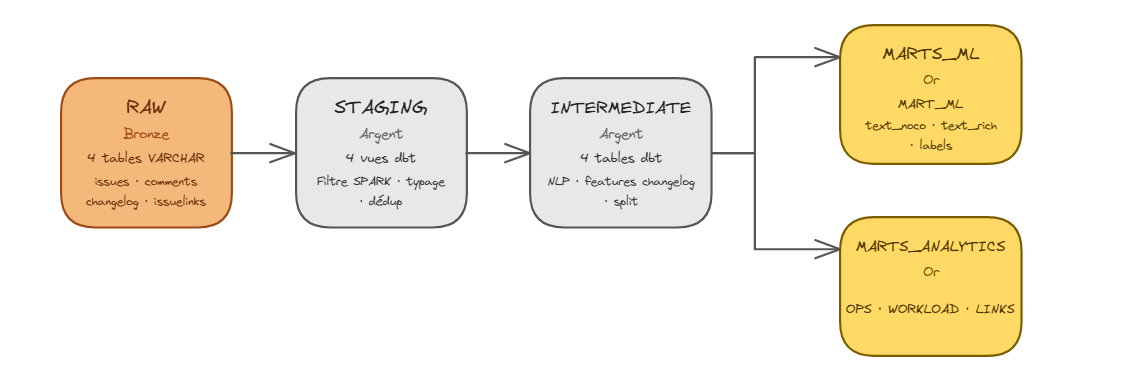
\includegraphics[width=\textwidth]{images/medallion_flow.png}
    \caption{Architecture en médaillon du processus de traitement}
    \label{fig:medallion_flow}
\end{figure}

\subsection{Couche Bronze : ingestion brute}

La couche Bronze constitue le point d'entrée des données dans la plateforme. Les quatre fichiers CSV sources sont chargés dans Snowflake en deux étapes. La commande \texttt{PUT} transfère les fichiers compressés depuis le système de fichiers local vers le stage interne Snowflake. La commande \texttt{COPY INTO} exécute ensuite l'ingestion vers les tables cibles. Toutes les colonnes sont stockées au format \texttt{VARCHAR}, reproduisant fidèlement la structure CSV d'origine grâce à un mapping positionnel (\texttt{\$N}). Aucune transformation métier n'est appliquée à ce stade, préservant ainsi un historique immuable qui permet de retraiter les couches supérieures à tout moment sans dépendre de la source originale.

\subsection{Couche Argent — Staging : filtrage mécanique}

La couche Staging est implémentée sous forme de vues dbt directement au-dessus des tables Bronze. Son rôle est de réaliser un ensemble d'opérations mécaniques de préparation : filtrage des tickets au seul projet Apache Spark, renommage des colonnes selon les conventions du projet, transtypage vers les types natifs Snowflake (entiers, dates, booléens) et déduplication. Pour le journal de modifications, un filtre supplémentaire est appliqué afin de ne retenir que les changements portant sur les champs métier pertinents : statut, priorité, résolution, assignataire et type d'incident. Ce filtrage réduit le volume du changelog de 9,6 millions à environ 400 000 entrées exploitables.

\subsection{Couche Argent — Intermédiaire : logique métier et ingénierie des caractéristiques}

La couche Intermédiaire porte l'essentiel de la valeur ajoutée du processus de traitement. Elle est implémentée sous forme de tables dbt matérialisées, calculées à partir des vues de Staging.

\subsubsection{Nettoyage textuel et normalisation des étiquettes}

Le modèle \textit{INT\_ISSUES\_CLEANED} applique une macro dbt de nettoyage NLP en six étapes successives sur les champs textuels : suppression des balises HTML, retrait des blocs de code délimités par des backticks, élimination des mentions d'utilisateurs (format @username), suppression des URLs, normalisation des espaces multiples, et mise en minuscule. En parallèle, les étiquettes brutes de type et de résolution sont remplacées par leurs valeurs normalisées via les seeds dbt \textit{issuetype\_mapping} et \textit{resolution\_mapping}. Enfin, une colonne \textit{split} est calculée pour chaque ticket selon sa date de création, affectant la valeur \textit{train} (avant 2022), \textit{val} (2022) ou \textit{test} (2023).

\subsubsection{Agrégation des commentaires}

Le modèle \textit{INT\_COMMENTS\_AGGREGATED} consolide les commentaires de chaque ticket selon la politique « premiers 5 + derniers 3 ». Cette heuristique capture à la fois le contexte initial de signalement, généralement exprimé dans les premiers échanges, et les éléments de résolution, qui apparaissent naturellement en fin de fil de discussion. Le texte agrégé résultant est intégré dans la vue enrichie du ticket (\textit{text\_rich}), qui constitue la seconde entrée du pipeline d'embedding.

\subsubsection{Extraction des caractéristiques du journal de modifications}

Le modèle \textit{INT\_CHANGELOG\_FEATURES} extrait des indicateurs comportementaux à partir du journal des modifications. L'indicateur \textit{was\_escalated} détecte si la priorité d'un ticket a été revue à la hausse au cours de son cycle de vie. Son calcul repose sur un mapping des étiquettes de priorité vers des entiers ordonnés (Blocker~=~4, Critical~=~3, Major~=~2, Minor~=~1, Trivial~=~0), permettant une comparaison numérique correcte que la comparaison alphabétique des chaînes de caractères ne permettrait pas. L'indicateur complémentaire \textit{was\_deescalated} capte le phénomène de baisse de priorité. L'indicateur \textit{n\_assignee\_changes} comptabilise le nombre de réassignations successives, signal révélateur de la complexité ou de l'ambiguïté du ticket. Ces caractéristiques sont utilisées comme signal de reranking dans le pipeline de classification.

\subsubsection{Caractéristiques des liens inter-tickets}

Le modèle \textit{INT\_ISSUELINKS\_FEATURES} calcule pour chaque ticket le nombre total de liens entrants et sortants ainsi que la distribution par type de lien (blocks, duplicates, relates to). Ces métriques fournissent une mesure de la connectivité du ticket dans le graphe des incidents, un signal complémentaire aux informations textuelles.

\subsection{Couche Or : tables de consommation}

La couche Or produit les tables finales destinées à la consommation par le pipeline de classification et par les applications de restitution.

\subsubsection{Mart Machine Learning}

La table \textit{MART\_ML}, hébergée dans le schéma \textit{MARTS\_ML}, constitue le contrat d'interface entre la couche de transformation et le pipeline Python. Elle consolide, pour chaque ticket, deux représentations textuelles complémentaires :

\begin{itemize}
    \item \textbf{text\_noco} : vue minimale du ticket composée du résumé, de la priorité, du statut et du reporter, sans aucune information pouvant agir comme indice sur l'étiquette cible. Cette représentation est conçue pour capturer l'essence du problème signalé.
    \item \textbf{text\_rich} : vue enrichie intégrant les commentaires agrégés et les métadonnées structurées (nombre de commentaires, nombre de liens, indicateurs de changelog). Cette représentation vise à capturer le contexte de résolution.
\end{itemize}

La table inclut également les étiquettes normalisées (\textit{issuetype\_norm}, \textit{resolution\_norm}), la colonne \textit{split} pour le découpage train/validation/test, et les caractéristiques numériques de changelog.

\subsubsection{Marts Analytiques}

Trois tables sont produites dans le schéma \textit{MARTS\_ANALYTICS} pour alimenter le tableau de bord :

\begin{itemize}
    \item \textbf{MART\_ANALYTICS\_OPS} : agrégats mensuels par type d'incident, couvrant l'ensemble des années disponibles sans restriction au seul ensemble d'entraînement.
    \item \textbf{MART\_ANALYTICS\_WORKLOAD} : métriques de charge par assignataire (volume de tickets assignés, délai médian de résolution, taux de clôture).
    \item \textbf{MART\_ANALYTICS\_LINKS} : métriques de connectivité par ticket (degré de liens entrants et sortants, présence de liens de blocage).
\end{itemize}

\subsection{Garanties de qualité}

L'ensemble du pipeline de transformation est couvert par une suite de plus de 50 tests dbt automatisés, répartis sur toutes les couches. Ces tests vérifient l'unicité des clés primaires, l'absence de valeurs nulles sur les colonnes critiques, la conformité des étiquettes normalisées aux valeurs attendues (incluant la valeur "Won't Fix"), et des contraintes de plage pour les indicateurs numériques. L'exécution de la commande \texttt{dbt test} produit un résultat sans aucun avertissement ni erreur, garantissant l'intégrité de la donnée à chaque étape du processus.

%--------------------------4-----------------------------
\section{Architecture générale du système}

\subsection{Vue d'ensemble}

La plateforme se décompose en quatre blocs fonctionnels qui s'articulent de manière séquentielle : la couche d'ingestion, la couche de transformation décrite dans la section précédente, le pipeline de classification hybride fondé sur l'intelligence artificielle, et la couche de restitution. La figure \ref{fig:archi_generale} illustre les flux de données entre ces composants et positionne chaque brique technologique dans l'architecture globale.

\begin{figure}[H]
    \centering
    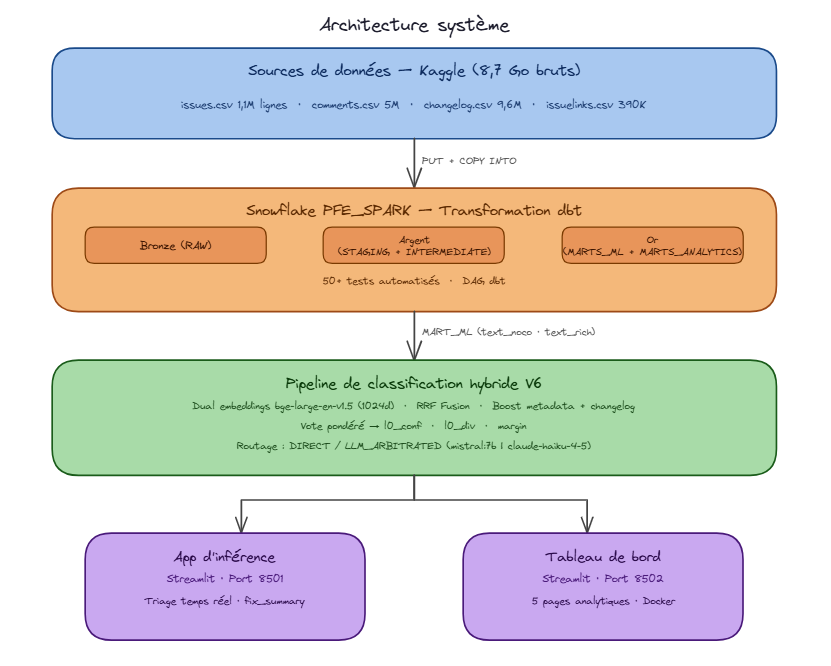
\includegraphics[width=\textwidth]{images/architecture_generale.png}
    \caption{Architecture générale de la plateforme de triage automatique}
    \label{fig:archi_generale}
\end{figure}

\subsection{Composants d'intelligence artificielle : vue d'ensemble}

L'intelligence artificielle intervient à plusieurs niveaux dans la plateforme, tous opérés exclusivement via \textbf{Snowflake Cortex} depuis des requêtes SQL. Cette intégration native garantit que les données ne quittent jamais l'environnement sécurisé Snowflake, ce qui est déterminant dans un contexte de conformité et de gouvernance des données.

Quatre fonctions Cortex sont mobilisées de manière combinée tout au long du pipeline :

\begin{itemize}
    \item \texttt{SNOWFLAKE.CORTEX.COMPLETE('mistral-large2', ...)} pour la summarization technique et l'extraction de mots clés, en raison de son excellent rapport performances/coût sur les tâches de génération structurée en anglais technique.
    \item \texttt{SNOWFLAKE.CORTEX.EMBED\_TEXT\_768('snowflake-arctic-embed-m', ...)} pour le calcul des vecteurs denses de 768 dimensions, natif à Snowflake et optimisé pour la recherche sémantique.
    \item \texttt{VECTOR\_COSINE\_SIMILARITY()} pour la recherche des tickets historiques les plus similaires, directement en SQL, sans bibliothèque externe ni infrastructure dédiée.
    \item \texttt{SNOWFLAKE.CORTEX.COMPLETE('llama3.3-70b', ...)} pour la classification finale par raisonnement few-shot et la génération des résumés correctifs, en raison de sa supériorité sur les prompts complexes avec chain-of-thought.
\end{itemize}

\subsection{Pipeline de classification RAG sur Snowflake Cortex}

Le pipeline de classification constitue le cœur intelligent du système. Il s'articule en cinq étapes séquentielles entièrement implémentées en SQL sur Snowflake, selon une architecture RAG (Retrieval-Augmented Generation) adaptée au contexte du triage de tickets. La figure \ref{fig:rag_archi} illustre le flux global du pipeline.

\begin{figure}[H]
    \centering
    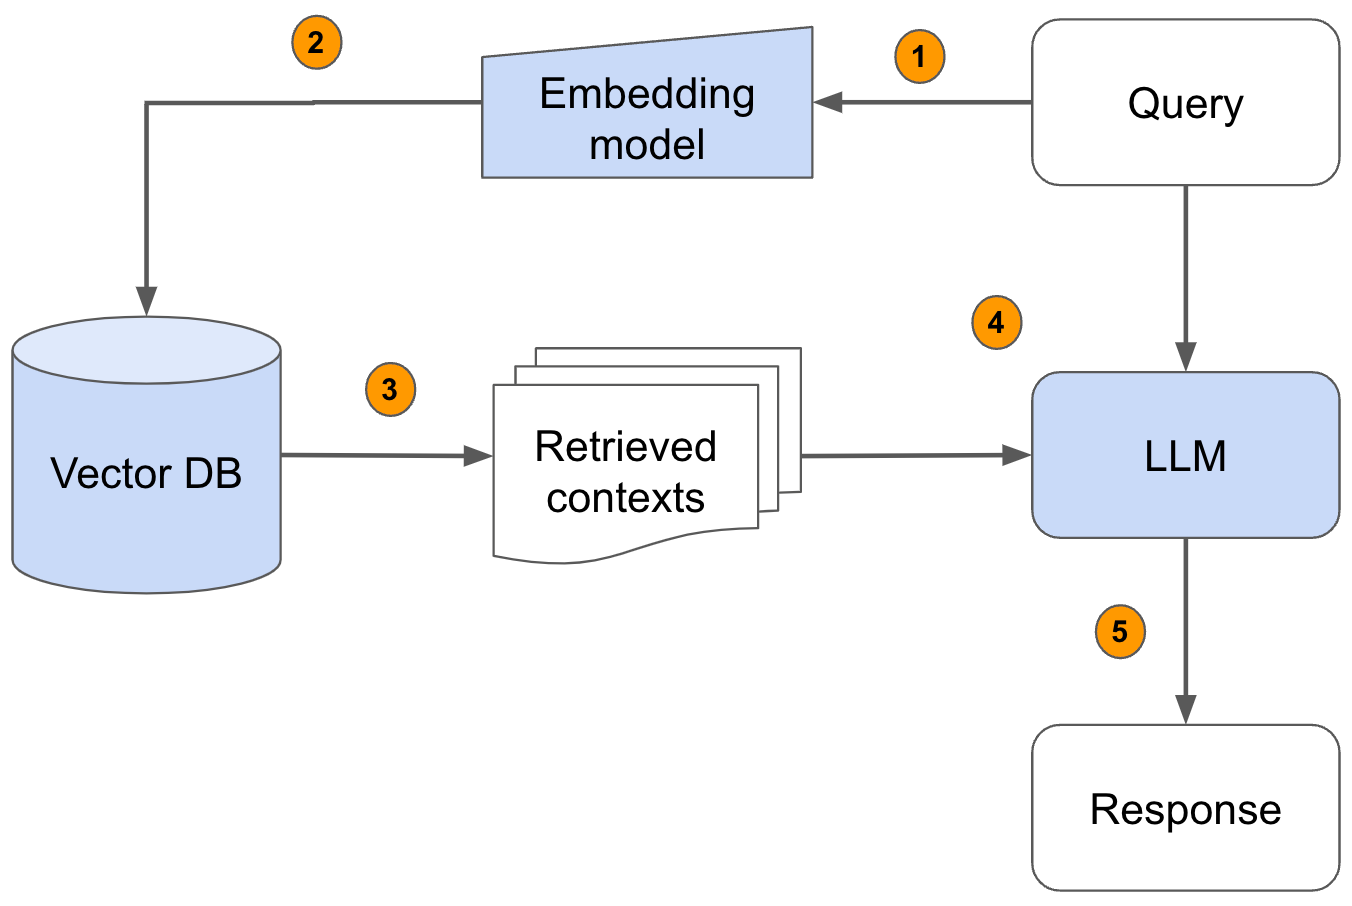
\includegraphics[width=0.85\textwidth]{images/rag_archi.png}
    \caption{Pipeline RAG de classification sur Snowflake Cortex}
    \label{fig:rag_archi}
\end{figure}

\subsubsection{Étape 1 — Construction du texte technique enrichi}

La première étape consiste à construire, pour chaque ticket de la base d'entraînement, une représentation textuelle unifiée à partir des sources disponibles. Les modèles dbt de la couche intermédiaire ont déjà produit les colonnes \textit{text\_noco} et \textit{text\_rich}. Ces représentations sont consolidées dans deux colonnes complémentaires utilisées par les étapes suivantes :

\begin{itemize}
    \item \textbf{INFORMATION\_ONE} : concaténation du résumé nettoyé, de la description et des commentaires agrégés (politique premiers-5 + derniers-3). Cette colonne sert de base pour le calcul des embeddings et les règles de correspondance lexicale.
    \item \textbf{INFORMATION\_TWO} : version étendue intégrant les métadonnées structurées (priorité, statut, indicateurs de changelog). Cette colonne est injectée dans le contexte du prompt LLM final pour enrichir le raisonnement du modèle.
\end{itemize}

Le recours aux commentaires est motivé par leur richesse informationnelle : les premiers commentaires exposent le contexte de signalement du problème, tandis que les derniers contiennent généralement les éléments menant à la résolution, deux signaux complémentaires pour la prédiction du type d'incident et de la résolution probable.

\subsubsection{Étape 2 — Summarization technique et embedding 768 dimensions}

La deuxième étape transforme chaque ticket en une représentation vectorielle dense via un processus en deux temps.

\paragraph{Summarization technique par LLM}

Avant de calculer l'embedding, une étape de summarization est appliquée via \texttt{CORTEX.COMPLETE('mistral-large2', ...)}. Un prompt personnalisé demande au modèle de supprimer tout le bruit du texte brut (balises HTML, URLs, références de tickets, adresses email) et de produire un résumé technique de 3 à 5 phrases ne conservant que le contenu discriminant : le composant défaillant, le système concerné et le comportement observé.

Cette étape est préférée à la fonction native \texttt{CORTEX.SUMMARIZE()} car cette dernière est généraliste et conserve les éléments de bruit. Le prompt personnalisé produit un texte standardisé, plus propre pour l'embedding et comparable entre tickets de styles rédactionnels très différents.

\paragraph{Calcul des embeddings 768D}

Le résumé nettoyé est ensuite encodé par le modèle \texttt{snowflake-arctic-embed-m} via la fonction \texttt{CORTEX.EMBED\_TEXT\_768()}, produisant un vecteur de 768 dimensions stocké nativement dans une colonne de type \texttt{VECTOR(FLOAT, 768)} :

\begin{lstlisting}[language=SQL]
SNOWFLAKE.CORTEX.EMBED_TEXT_768(
    'snowflake-arctic-embed-m',
    COALESCE(SUMMARIZED_ONE, LEFT(INFORMATION_ONE, 512))
) AS EMBEDDING_ONE
\end{lstlisting}

Le \texttt{COALESCE} protège contre les cas où la summarization échoue, en utilisant directement les 512 premiers caractères du texte brut. Les embeddings calculés constituent la base vectorielle de référence du système RAG.

Le choix du modèle \texttt{snowflake-arctic-embed-m} est justifié par trois facteurs convergents : son intégration native dans Snowflake sans aucun transfert de données, ses 768 dimensions offrant un bon équilibre entre précision sémantique et coût de stockage, et ses performances de premier plan sur les tâches de recherche sémantique en anglais technique.

\subsubsection{Étape 3 — Extraction de mots clés techniques}

La troisième étape enrichit chaque ticket d'un ensemble de mots clés techniques extraits par LLM. Un prompt \texttt{mistral-large2} demande au modèle d'extraire les dix termes les plus discriminants du texte du ticket, en se concentrant sur les noms de technologies, de composants, de types d'erreurs et de systèmes impliqués. Ces mots clés sont ensuite agrégés par catégorie cible (\textit{issuetype\_norm}) pour construire un dictionnaire de signatures textuelles : les termes les plus fréquents dans les tickets d'une catégorie constituent son empreinte lexicale distinctive.

La motivation de cette étape est de corriger un biais structurel de la similarité cosinus : deux tickets peuvent être sémantiquement proches sans partager les mêmes termes techniques discriminants. Un ticket mentionnant un \textit{NullPointerException dans le planificateur de tâches} et un ticket évoquant une \textit{exception dans le gestionnaire de ressources} peuvent avoir une forte similarité vectorielle mais relever de catégories différentes. Les mots clés apportent un signal lexical complémentaire au signal sémantique.

\subsubsection{Étape 4 — Recherche par similarité et re-ranking hybride}

La quatrième étape constitue le cœur du pipeline RAG. Pour chaque ticket de validation, le système recherche les tickets d'entraînement les plus similaires, puis re-ranke les résultats par un score hybride combinant similarité sémantique et correspondance de mots clés.

\paragraph{Recherche par similarité cosinus}

Le ticket de validation est d'abord encodé par le même modèle d'embedding que les tickets d'entraînement, garantissant la cohérence de l'espace vectoriel. Il est ensuite comparé à l'ensemble de la base d'entraînement via \texttt{VECTOR\_COSINE\_SIMILARITY()} en SQL. Pour deux vecteurs $\mathbf{a}$ et $\mathbf{b}$ de dimension 768, la similarité cosinus est définie par :

$$\text{sim}(\mathbf{a}, \mathbf{b}) = \frac{\mathbf{a} \cdot \mathbf{b}}{\|\mathbf{a}\| \cdot \|\mathbf{b}\|}$$

Cette métrique est insensible à la norme des vecteurs et mesure uniquement l'alignement directionnel dans l'espace sémantique, ce qui la rend particulièrement robuste aux variations de longueur des textes. Les cinq tickets d'entraînement présentant le score de similarité cosinus le plus élevé sont retenus comme candidats initiaux.

\paragraph{Re-ranking hybride sémantique + mots clés}

Le classement initial est ensuite affiné par un score combiné :

$$\text{COMBINED\_SCORE} = (\text{SIMILARITY\_SCORE} \times 0{,}6) + (\text{keyword\_match\_count} \times 0{,}08)$$

Le \textit{keyword\_match\_count} comptabilise le nombre de mots clés caractéristiques de la catégorie candidate présents dans le texte du ticket à classifier. Ce re-ranking peut inverser le classement initial : un ticket candidat avec une similarité cosinus légèrement inférieure mais partageant davantage de termes techniques discriminants avec la requête remonte dans le classement final.

\subsubsection{Étape 5 — Classification par LLM avec few-shot dynamique}

La cinquième étape soumet les résultats du re-ranking à \texttt{llama3.3-70b} pour produire la prédiction finale. Le modèle \texttt{llama3.3-70b} est retenu pour sa supériorité sur les prompts complexes avec chain-of-thought par rapport à \texttt{mistral-large2}, et pour sa meilleure capacité à suivre des instructions détaillées portant sur plusieurs catégories avec des règles de désambiguïsation explicites.

Un prompt structuré en cinq couches est construit dynamiquement pour chaque ticket :

\begin{enumerate}
    \item \textbf{Définitions des catégories} : toutes les valeurs valides de \textit{issuetype\_norm} et \textit{resolution\_norm} avec leur description, permettant au modèle de comprendre les nuances entre catégories voisines (ex : Bug vs Improvement lorsque le ticket propose un correctif).
    \item \textbf{Règles de désambiguïsation} : construites par analyse des erreurs sur le jeu de validation, ces règles encodent les confusions fréquentes observées empiriquement.
    \item \textbf{Few-shot dynamique re-ranké} : les cinq exemples issus du re-ranking, présentés avec leurs scores de similarité et de correspondance de mots clés, ainsi que leurs étiquettes cibles connues.
    \item \textbf{Catégories candidates restreintes} : seules les catégories effectivement représentées dans le top-5 sont soumises au choix du modèle, réduisant l'espace de décision et améliorant la précision.
    \item \textbf{Chain-of-thought} : une instruction explicite demande au modèle de raisonner en plusieurs étapes avant de formuler sa réponse finale.
\end{enumerate}

La réponse du modèle est ensuite validée syntaxiquement : si la valeur retournée ne correspond pas exactement à l'une des catégories valides, un mécanisme de normalisation par correspondance partielle (\texttt{ILIKE}) la corrige vers la catégorie la plus proche, garantissant que la sortie finale est toujours une étiquette reconnue.

\subsection{Génération des résumés correctifs}

Pour chaque ticket classifié, le pipeline génère un résumé correctif de 1 à 2 phrases décrivant l'analyse de la cause probable de l'incident. Ce résumé est généré par \texttt{llama3.3-70b} dans une requête séparée, \textit{après} que la classification est définitivement fixée. Cette séquentialité est délibérée : générer le résumé dans la même requête que la classification créerait un biais circulaire où le modèle pourrait être influencé par le résumé qu'il est en train de produire, au détriment de la fiabilité de l'étiquette prédite.

Le prompt de génération reçoit le type d'incident prédit, le texte du ticket, le domaine applicatif et la priorité. Il est instruit de commencer par \textit{«~L'incident a été causé par...~»} et de mentionner le composant ou le module spécifique impliqué. La concision maximale (1-2 phrases) garantit des résumés directement exploitables par les équipes de développement, sans nécessiter de reformulation.

\subsection{Couche de restitution}

La plateforme expose deux applications Streamlit pour la restitution des résultats aux utilisateurs finaux.

\subsubsection{Application de triage en temps réel}

L'application d'inférence, accessible sur le port 8501, permet le triage en temps réel d'un nouveau ticket. L'utilisateur saisit le résumé et la description du ticket. L'application appelle le pipeline Cortex SQL, puis affiche la prédiction du type d'incident, la résolution probable et le résumé correctif. Un panneau dédié présente les tickets historiques les plus similaires avec leurs scores de similarité et de correspondance de mots clés, offrant aux développeurs un point de départ concret pour la résolution du problème signalé.

\subsubsection{Tableau de bord analytique}

L'application analytique, accessible sur le port 8502, est une application multi-pages permettant l'exploration des données opérationnelles historiques. Elle est structurée en cinq pages complémentaires alimentées par les tables \textit{MART\_ANALYTICS\_OPS}, \textit{MART\_ANALYTICS\_WORKLOAD} et \textit{MART\_ANALYTICS\_LINKS} :

\begin{itemize}
    \item \textbf{Page 1 — Vue d'ensemble} : évolution mensuelle du volume de tickets et répartition par type d'incident.
    \item \textbf{Page 2 — Résolution} : analyse des délais de résolution et distribution des motifs de clôture.
    \item \textbf{Page 3 — Charge de travail} : tableau de bord par assignataire (volume, délai médian, taux de clôture).
    \item \textbf{Page 4 — Relations} : exploration des liens entre tickets et identification des composants les plus bloquants.
    \item \textbf{Page 5 — Anomalies} : détection de tickets présentant des patterns de changelog anormaux (forte rotation d'assignataires, escalades de priorité, délais de résolution atypiques).
\end{itemize}

%--------------------------5-----------------------------
\section{Conclusion}

Ce chapitre a posé les fondations de la conception de la plateforme de triage automatique. Nous avons présenté le jeu de données Apache JIRA dans sa structure, son volume et ses spécificités, avant de décrire en détail le processus de transformation qui, à travers l'architecture en médaillon pilotée par dbt, produit des tables de consommation fiables et validées par plus de 50 tests automatisés. Nous avons ensuite décrit l'architecture générale du système et détaillé le pipeline RAG implémenté entièrement sur Snowflake Cortex : summarization par \texttt{mistral-large2}, embedding 768 dimensions par \texttt{snowflake-arctic-embed-m}, re-ranking hybride sémantique et mots clés, classification few-shot par \texttt{llama3.3-70b} avec chain-of-thought, et génération de résumés correctifs. Le chapitre suivant sera consacré à la réalisation et à la mise en œuvre de cette architecture, en présentant les aspects d'implémentation et les résultats obtenus sur l'ensemble de test.

        \chapter{Réalisation et mise en œuvre}
\rhead{Réalisation et mise en œuvre}

%+++++++++++++++++Introduction+++++++++++%
\section{Introduction}


%+++++++++++++++++Outils+++++++++++%
\section{Environnement technique et outils utilisés}
\begin{minipage}{0.7\textwidth}
    \textbf{Visual Studio Code:} est un éditeur de code source qui peut être utilisé avec une variété de langages de programmation, notamment Java, JavaScript, Go, Node.js et C++. Il est basé sur le cadre Electron, qui est utilisé pour développer des applications Web Node.js qui s’exécutent sur le moteur de présentation Blink. Visual Studio Code utilise le même composant d’éditeur (nom de code Monaco) utilisé dans Azure DevOps (anciennement appelé Visual Studio Online et Visual Studio Team Services).
\end{minipage}
\hfill
\begin{minipage}{0.3\textwidth}
    \centering
    
\includegraphics[width=0.4\linewidth]{images/Visual_Studio.png}
    \captionof{figure}{Visual Studio Code}
\end{minipage}

\vspace{1.2cm}

\begin{minipage}{0.7\textwidth}
    \textbf{Snowflake:} est une plateforme de données cloud qui fonctionne comme un entrepôt de données en tant que service (DWaaS). Elle se distingue par une architecture qui sépare le stockage, le calcul et les services de gestion en trois couches indépendantes, permettant de les dimensionner séparément selon les besoins. Snowflake prend en charge les requêtes SQL, les données semi-structurées et offre des fonctionnalités telles que le clonage instantané, le partage de données entre organisations et la réplication multi-cloud.
\end{minipage}
\hfill
\begin{minipage}{0.3\textwidth}
    \centering
    
\includegraphics[width=0.75\linewidth]{images/snowflake.jpg}
    \captionof{figure}{Snowflake}
\end{minipage}

\vspace{1.2cm}

\begin{minipage}{0.7\textwidth}
    \textbf{Cortex:} est un service d'intelligence artificielle intégré nativement à la plateforme Snowflake. Il permet d'exécuter des modèles de langage et de calculer des embeddings vectoriels directement depuis des requêtes SQL, sans que les données ne quittent l'environnement Snowflake
\end{minipage}
\hfill
\begin{minipage}{0.3\textwidth}
    \centering
    
\includegraphics[width=0.7\linewidth]{images/cortex.png}
    \captionof{figure}{Cortex}
\end{minipage}

\vspace{1.2cm}

\begin{minipage}{0.7\textwidth}
    \textbf{Python :} est un langage de programmation interprété, facile à lire et à écrire, connu pour sa simplicité et sa polyvalence. Il est largement utilisé dans de nombreux domaines comme le développement web, l’analyse de données, l’intelligence artificielle, la robotique et l’automatisation. Grâce à sa large communauté et à ses nombreuses bibliothèques, Python est devenu l’un des langages les plus populaires aujourd’hui.
\end{minipage}
\hfill
\begin{minipage}{0.3\textwidth}
    \centering
    
\includegraphics[width=0.5\linewidth]{images/python.png}
    \captionof{figure}{Python}
\end{minipage}

\vspace{1.2cm}

\begin{minipage}{0.7\textwidth}
    \textbf{Streamlit:} est un framework open-source en Python qui permet de créer facilement des applications web interactives pour la data science et le machine learning. Il suffit d’écrire du code Python simple pour transformer des scripts en interfaces web intuitives, sans avoir besoin de connaissances en développement web.
\end{minipage}
\hfill
\begin{minipage}{0.3\textwidth}
    \centering
    
\includegraphics[width=0.5\linewidth]{images/streamlit.png}
    \captionof{figure}{Streamlit}
\end{minipage}

\vspace{1.2cm}

\begin{minipage}{0.7\textwidth}
    \textbf{PowerBI:} est une solution de Business Intelligence développée par Microsoft qui permet de se connecter à diverses sources de données, de les transformer et de les visualiser sous forme de tableaux de bord interactifs. Elle repose sur le langage DAX pour les mesures calculées et le moteur Power Query pour la préparation des données. Power BI offre également un service cloud pour la publication et le partage de rapports au sein d'une organisation.
\end{minipage}
\hfill
\begin{minipage}{0.3\textwidth}
    \centering
    
\includegraphics[width=0.7\linewidth]{images/powerbi.jpg}
    \captionof{figure}{PowerBI}
\end{minipage}

\vspace{1.2cm}

\begin{minipage}{0.7\textwidth}
    \textbf{Apache Airflow:} Airflow est un outil open source de gestion et d’orchestration de workflows.
    Il permet de planifier, d’automatiser et de suivre des chaînes complexes de tâches (pipelines de données), en assurant leur exécution dans un ordre précis et en gérant les dépendances entre elles.
\end{minipage}
\hfill
\begin{minipage}{0.3\textwidth}
    \centering
    
\includegraphics[width=0.55\linewidth]{images/airflow.png}
    \captionof{figure}{Airflow}
\end{minipage}


%++++++++++++++++Implémentation+++++++++++%
\section{Implémentation détaillée}


%+++++++++++++++++Resultat+++++++++++%
\section{Tests et validation des résultats}


%+++++++++++++++++Conclusion+++++++++++%
\section{Conclusion}



    % Webographie
\addcontentsline{toc}{chapter}{Webographie}

     \printbibliography


    \newpage
    
    


\end{document}







